% Options for packages loaded elsewhere
\PassOptionsToPackage{unicode}{hyperref}
\PassOptionsToPackage{hyphens}{url}
%
\documentclass[
]{book}
\usepackage{amsmath,amssymb}
\usepackage{iftex}
\ifPDFTeX
  \usepackage[T1]{fontenc}
  \usepackage[utf8]{inputenc}
  \usepackage{textcomp} % provide euro and other symbols
\else % if luatex or xetex
  \usepackage{unicode-math} % this also loads fontspec
  \defaultfontfeatures{Scale=MatchLowercase}
  \defaultfontfeatures[\rmfamily]{Ligatures=TeX,Scale=1}
\fi
\usepackage{lmodern}
\ifPDFTeX\else
  % xetex/luatex font selection
\fi
% Use upquote if available, for straight quotes in verbatim environments
\IfFileExists{upquote.sty}{\usepackage{upquote}}{}
\IfFileExists{microtype.sty}{% use microtype if available
  \usepackage[]{microtype}
  \UseMicrotypeSet[protrusion]{basicmath} % disable protrusion for tt fonts
}{}
\makeatletter
\@ifundefined{KOMAClassName}{% if non-KOMA class
  \IfFileExists{parskip.sty}{%
    \usepackage{parskip}
  }{% else
    \setlength{\parindent}{0pt}
    \setlength{\parskip}{6pt plus 2pt minus 1pt}}
}{% if KOMA class
  \KOMAoptions{parskip=half}}
\makeatother
\usepackage{xcolor}
\usepackage{color}
\usepackage{fancyvrb}
\newcommand{\VerbBar}{|}
\newcommand{\VERB}{\Verb[commandchars=\\\{\}]}
\DefineVerbatimEnvironment{Highlighting}{Verbatim}{commandchars=\\\{\}}
% Add ',fontsize=\small' for more characters per line
\usepackage{framed}
\definecolor{shadecolor}{RGB}{248,248,248}
\newenvironment{Shaded}{\begin{snugshade}}{\end{snugshade}}
\newcommand{\AlertTok}[1]{\textcolor[rgb]{0.94,0.16,0.16}{#1}}
\newcommand{\AnnotationTok}[1]{\textcolor[rgb]{0.56,0.35,0.01}{\textbf{\textit{#1}}}}
\newcommand{\AttributeTok}[1]{\textcolor[rgb]{0.13,0.29,0.53}{#1}}
\newcommand{\BaseNTok}[1]{\textcolor[rgb]{0.00,0.00,0.81}{#1}}
\newcommand{\BuiltInTok}[1]{#1}
\newcommand{\CharTok}[1]{\textcolor[rgb]{0.31,0.60,0.02}{#1}}
\newcommand{\CommentTok}[1]{\textcolor[rgb]{0.56,0.35,0.01}{\textit{#1}}}
\newcommand{\CommentVarTok}[1]{\textcolor[rgb]{0.56,0.35,0.01}{\textbf{\textit{#1}}}}
\newcommand{\ConstantTok}[1]{\textcolor[rgb]{0.56,0.35,0.01}{#1}}
\newcommand{\ControlFlowTok}[1]{\textcolor[rgb]{0.13,0.29,0.53}{\textbf{#1}}}
\newcommand{\DataTypeTok}[1]{\textcolor[rgb]{0.13,0.29,0.53}{#1}}
\newcommand{\DecValTok}[1]{\textcolor[rgb]{0.00,0.00,0.81}{#1}}
\newcommand{\DocumentationTok}[1]{\textcolor[rgb]{0.56,0.35,0.01}{\textbf{\textit{#1}}}}
\newcommand{\ErrorTok}[1]{\textcolor[rgb]{0.64,0.00,0.00}{\textbf{#1}}}
\newcommand{\ExtensionTok}[1]{#1}
\newcommand{\FloatTok}[1]{\textcolor[rgb]{0.00,0.00,0.81}{#1}}
\newcommand{\FunctionTok}[1]{\textcolor[rgb]{0.13,0.29,0.53}{\textbf{#1}}}
\newcommand{\ImportTok}[1]{#1}
\newcommand{\InformationTok}[1]{\textcolor[rgb]{0.56,0.35,0.01}{\textbf{\textit{#1}}}}
\newcommand{\KeywordTok}[1]{\textcolor[rgb]{0.13,0.29,0.53}{\textbf{#1}}}
\newcommand{\NormalTok}[1]{#1}
\newcommand{\OperatorTok}[1]{\textcolor[rgb]{0.81,0.36,0.00}{\textbf{#1}}}
\newcommand{\OtherTok}[1]{\textcolor[rgb]{0.56,0.35,0.01}{#1}}
\newcommand{\PreprocessorTok}[1]{\textcolor[rgb]{0.56,0.35,0.01}{\textit{#1}}}
\newcommand{\RegionMarkerTok}[1]{#1}
\newcommand{\SpecialCharTok}[1]{\textcolor[rgb]{0.81,0.36,0.00}{\textbf{#1}}}
\newcommand{\SpecialStringTok}[1]{\textcolor[rgb]{0.31,0.60,0.02}{#1}}
\newcommand{\StringTok}[1]{\textcolor[rgb]{0.31,0.60,0.02}{#1}}
\newcommand{\VariableTok}[1]{\textcolor[rgb]{0.00,0.00,0.00}{#1}}
\newcommand{\VerbatimStringTok}[1]{\textcolor[rgb]{0.31,0.60,0.02}{#1}}
\newcommand{\WarningTok}[1]{\textcolor[rgb]{0.56,0.35,0.01}{\textbf{\textit{#1}}}}
\usepackage{longtable,booktabs,array}
\usepackage{calc} % for calculating minipage widths
% Correct order of tables after \paragraph or \subparagraph
\usepackage{etoolbox}
\makeatletter
\patchcmd\longtable{\par}{\if@noskipsec\mbox{}\fi\par}{}{}
\makeatother
% Allow footnotes in longtable head/foot
\IfFileExists{footnotehyper.sty}{\usepackage{footnotehyper}}{\usepackage{footnote}}
\makesavenoteenv{longtable}
\usepackage{graphicx}
\makeatletter
\def\maxwidth{\ifdim\Gin@nat@width>\linewidth\linewidth\else\Gin@nat@width\fi}
\def\maxheight{\ifdim\Gin@nat@height>\textheight\textheight\else\Gin@nat@height\fi}
\makeatother
% Scale images if necessary, so that they will not overflow the page
% margins by default, and it is still possible to overwrite the defaults
% using explicit options in \includegraphics[width, height, ...]{}
\setkeys{Gin}{width=\maxwidth,height=\maxheight,keepaspectratio}
% Set default figure placement to htbp
\makeatletter
\def\fps@figure{htbp}
\makeatother
\setlength{\emergencystretch}{3em} % prevent overfull lines
\providecommand{\tightlist}{%
  \setlength{\itemsep}{0pt}\setlength{\parskip}{0pt}}
\setcounter{secnumdepth}{5}
\usepackage{booktabs}
\ifLuaTeX
  \usepackage{selnolig}  % disable illegal ligatures
\fi
\usepackage[]{natbib}
\bibliographystyle{plainnat}
\IfFileExists{bookmark.sty}{\usepackage{bookmark}}{\usepackage{hyperref}}
\IfFileExists{xurl.sty}{\usepackage{xurl}}{} % add URL line breaks if available
\urlstyle{same}
\hypersetup{
  pdftitle={Notions de statistiques},
  pdfauthor={Pascal Bessonneau},
  hidelinks,
  pdfcreator={LaTeX via pandoc}}

\title{Notions de statistiques}
\author{Pascal Bessonneau}
\date{2024-04-24}

\begin{document}
\maketitle

{
\setcounter{tocdepth}{1}
\tableofcontents
}
\hypertarget{statistiques-descriptives-et-tests}{%
\chapter{Statistiques descriptives et tests}\label{statistiques-descriptives-et-tests}}

Le but est de faire un peu de révision sur les statistiques descriptives et
les tests statistiques.

\hypertarget{statistiques-descriptives}{%
\chapter{Statistiques descriptives}\label{statistiques-descriptives}}

Le but de ce document est de rappeler les différents indicateurs utilisés dans
les statistiques descriptives.

\hypertarget{distribution}{%
\section{Distribution}\label{distribution}}

Dans le cas qualitatif, on appele \textbf{distribution} la répartition des
probabilités pour tous les points pour laquelle la distribution existe.

\begin{Shaded}
\begin{Highlighting}[]
\NormalTok{p }\OtherTok{\textless{}{-}} \FunctionTok{rbinom}\NormalTok{(}\AttributeTok{n=}\DecValTok{10000}\NormalTok{, }\AttributeTok{size =} \DecValTok{10}\NormalTok{,}\AttributeTok{p =} \FloatTok{0.2}\NormalTok{)}
\FunctionTok{barplot}\NormalTok{(}\FunctionTok{prop.table}\NormalTok{(}\FunctionTok{table}\NormalTok{(p)))}
\end{Highlighting}
\end{Shaded}

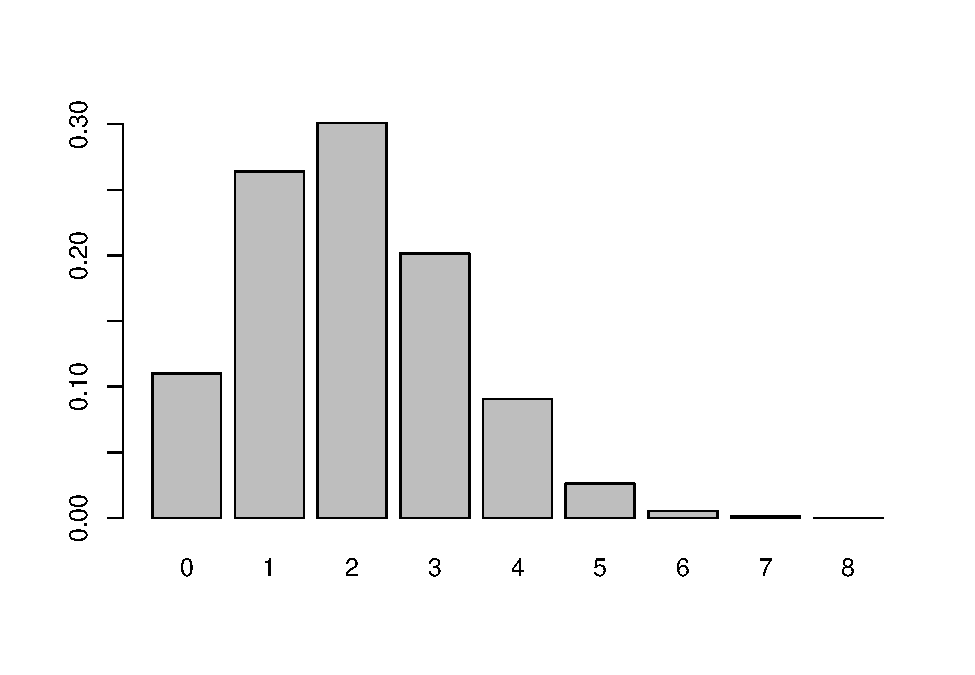
\includegraphics{_main_files/figure-latex/unnamed-chunk-2-1.pdf}

Nous voyons pour une distribution binomiale la distribution, cela représente
un lancer de dés avec ici, la somme de dix lancers, avec 0,2 la probabilité d'obtenir
un 1 et 0,8 la probabilité d'obtenir un 0. Ici la probabilité d'obtenir un score
de 3 est d'environ 20\%.

Dans le cas quantitatif, on appele \textbf{distribution} la répartition des
probabilités pour tous les points pour laquelle la distribution existe.
La plus connu est la loi normale:

\begin{Shaded}
\begin{Highlighting}[]
\NormalTok{exemple }\OtherTok{\textless{}{-}} \FunctionTok{rnorm}\NormalTok{(}\DecValTok{1000000}\NormalTok{,}\DecValTok{0}\NormalTok{,}\DecValTok{1}\NormalTok{)}
\FunctionTok{plot}\NormalTok{(}\FunctionTok{density}\NormalTok{(exemple),}\AttributeTok{main=}\StringTok{"Loi normale"}\NormalTok{,}\AttributeTok{ylab=}\StringTok{"Densité"}\NormalTok{)}
\end{Highlighting}
\end{Shaded}

La loi normale prends deux paramètres : l'écart-type et la moyenne.

Si on fait varier l'écart-type : on a une forme plus aplatie ou inversement.

\begin{Shaded}
\begin{Highlighting}[]
\FunctionTok{plot}\NormalTok{(}\FunctionTok{density}\NormalTok{(}\FunctionTok{rnorm}\NormalTok{(}\DecValTok{100000}\NormalTok{,}\DecValTok{0}\NormalTok{,}\FloatTok{0.5}\NormalTok{)),}\AttributeTok{main=}\StringTok{"Loi normale"}\NormalTok{,}\AttributeTok{ylab=}\StringTok{"Densité"}\NormalTok{)}
\FunctionTok{lines}\NormalTok{(}\FunctionTok{density}\NormalTok{(}\FunctionTok{rnorm}\NormalTok{(}\DecValTok{100000}\NormalTok{,}\DecValTok{0}\NormalTok{,}\DecValTok{1}\NormalTok{)),}\AttributeTok{main=}\StringTok{"Loi normale"}\NormalTok{,}\AttributeTok{ylab=}\StringTok{"Densité"}\NormalTok{)}
\FunctionTok{lines}\NormalTok{(}\FunctionTok{density}\NormalTok{(}\FunctionTok{rnorm}\NormalTok{(}\DecValTok{100000}\NormalTok{,}\DecValTok{0}\NormalTok{,}\FloatTok{1.5}\NormalTok{)),}\AttributeTok{main=}\StringTok{"Loi normale"}\NormalTok{,}\AttributeTok{ylab=}\StringTok{"Densité"}\NormalTok{)}
\FunctionTok{lines}\NormalTok{(}\FunctionTok{density}\NormalTok{(}\FunctionTok{rnorm}\NormalTok{(}\DecValTok{100000}\NormalTok{,}\DecValTok{0}\NormalTok{,}\DecValTok{2}\NormalTok{)),}\AttributeTok{main=}\StringTok{"Loi normale"}\NormalTok{,}\AttributeTok{ylab=}\StringTok{"Densité"}\NormalTok{)}
\end{Highlighting}
\end{Shaded}

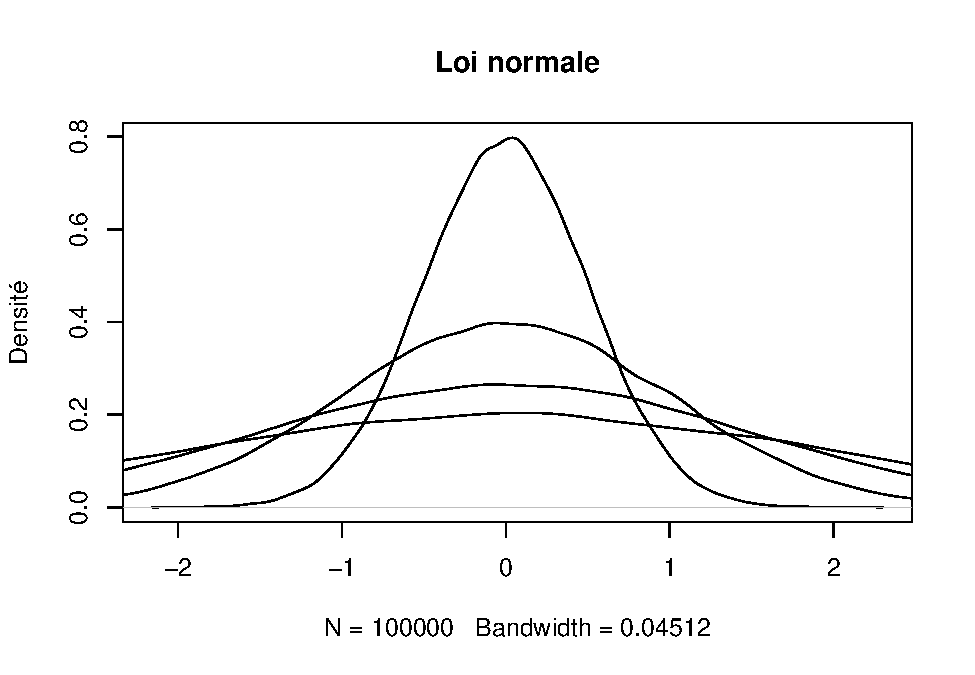
\includegraphics{_main_files/figure-latex/unnamed-chunk-4-1.pdf}

Si on fait varier la moyenne : la ``pointe'' de la courbe varie dans son
positionnement.

\begin{Shaded}
\begin{Highlighting}[]
\NormalTok{exemple }\OtherTok{\textless{}{-}} \FunctionTok{rnorm}\NormalTok{(}\DecValTok{1000000}\NormalTok{,}\DecValTok{0}\NormalTok{,}\DecValTok{1}\NormalTok{)}
\FunctionTok{plot}\NormalTok{(}\FunctionTok{density}\NormalTok{(exemple),}\AttributeTok{main=}\StringTok{"Loi normale"}\NormalTok{,}\AttributeTok{ylab=}\StringTok{"Densité"}\NormalTok{)}
\end{Highlighting}
\end{Shaded}

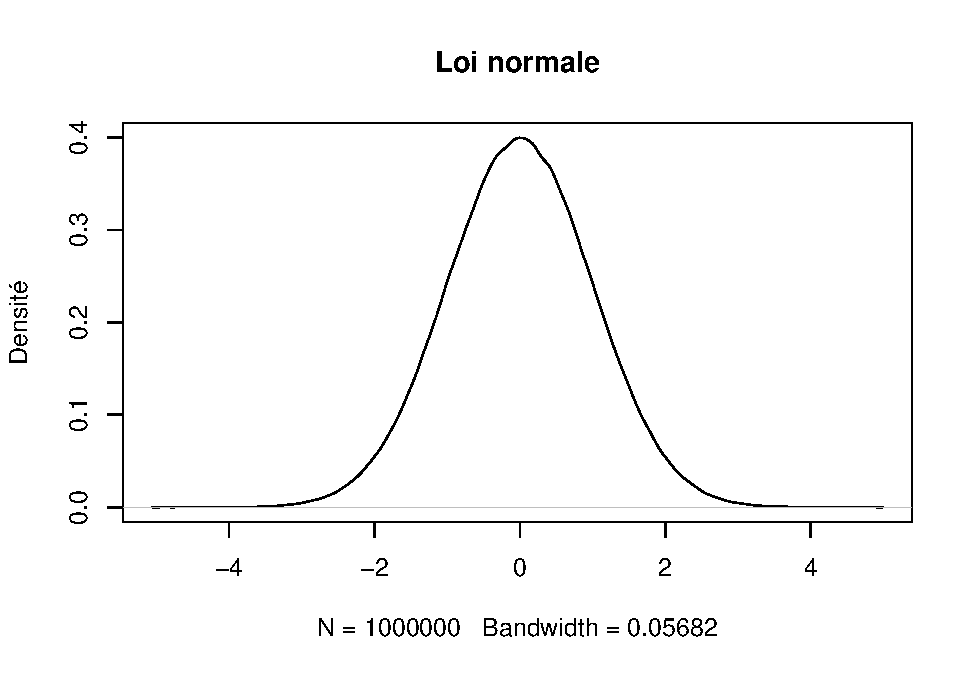
\includegraphics{_main_files/figure-latex/unnamed-chunk-5-1.pdf}

\hypertarget{indicateurs-de-position-mesures-de-tendance-centrale}{%
\section{Indicateurs de position (mesures de tendance centrale)}\label{indicateurs-de-position-mesures-de-tendance-centrale}}

La plupart des indicateurs statistiques s'inspire de la loi normale : Les indicateurs
de position donnent une idée de où se répartissent les points.

Le premier indicateur est la moyenne arithmétique, elle a de nombreux
prolongements en mathématiques, physique, etc.

Il y a des indicateurs proches comme la moyenne géométrique, la moyenne harmonique, etc.
La moyenne arithmétique est la plus utilisée.

\hypertarget{moyenne-arithmuxe9tqiue}{%
\subsection{Moyenne arithmétqiue}\label{moyenne-arithmuxe9tqiue}}

En statistiques, on retrouve cette moyenne dans l'ANOVA, la régression, le test de
Student, etc.

C'est celle qui se retrouve dans la plupart des cas dans les formules.

\begin{Shaded}
\begin{Highlighting}[]
\NormalTok{y}\OtherTok{=}\FunctionTok{rnorm}\NormalTok{(}\DecValTok{1000000}\NormalTok{,}\DecValTok{1}\NormalTok{,}\DecValTok{1}\NormalTok{)}
\FunctionTok{plot}\NormalTok{(}\FunctionTok{density}\NormalTok{(y),}\AttributeTok{main=}\StringTok{"Normale de moyenne 1"}\NormalTok{,}\AttributeTok{xlab=}\StringTok{"Valeurs de x"}\NormalTok{,}\AttributeTok{ylab=}\StringTok{"Densité"}\NormalTok{)}
\FunctionTok{abline}\NormalTok{(}\AttributeTok{v=}\DecValTok{1}\NormalTok{,}\AttributeTok{lty=}\DecValTok{3}\NormalTok{)}
\end{Highlighting}
\end{Shaded}

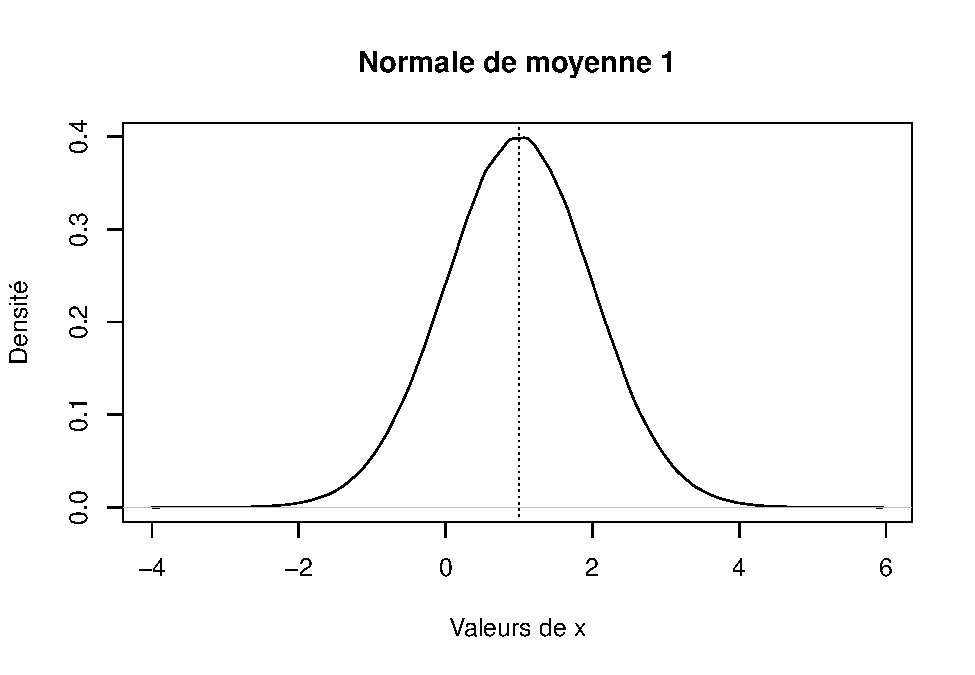
\includegraphics{_main_files/figure-latex/unnamed-chunk-6-1.pdf}

\begin{Shaded}
\begin{Highlighting}[]
\NormalTok{y}\OtherTok{=}\FunctionTok{rchisq}\NormalTok{(}\DecValTok{1000000}\NormalTok{,}\DecValTok{10}\NormalTok{)}
\FunctionTok{plot}\NormalTok{(}\FunctionTok{density}\NormalTok{(y),}\AttributeTok{main=}\StringTok{"Loi du Chi²"}\NormalTok{,}\AttributeTok{xlab=}\StringTok{"Valeurs de x"}\NormalTok{,}\AttributeTok{ylab=}\StringTok{"Densité"}\NormalTok{)}
\FunctionTok{abline}\NormalTok{(}\AttributeTok{v=}\FunctionTok{mean}\NormalTok{(y),}\AttributeTok{lty=}\DecValTok{3}\NormalTok{)}
\end{Highlighting}
\end{Shaded}

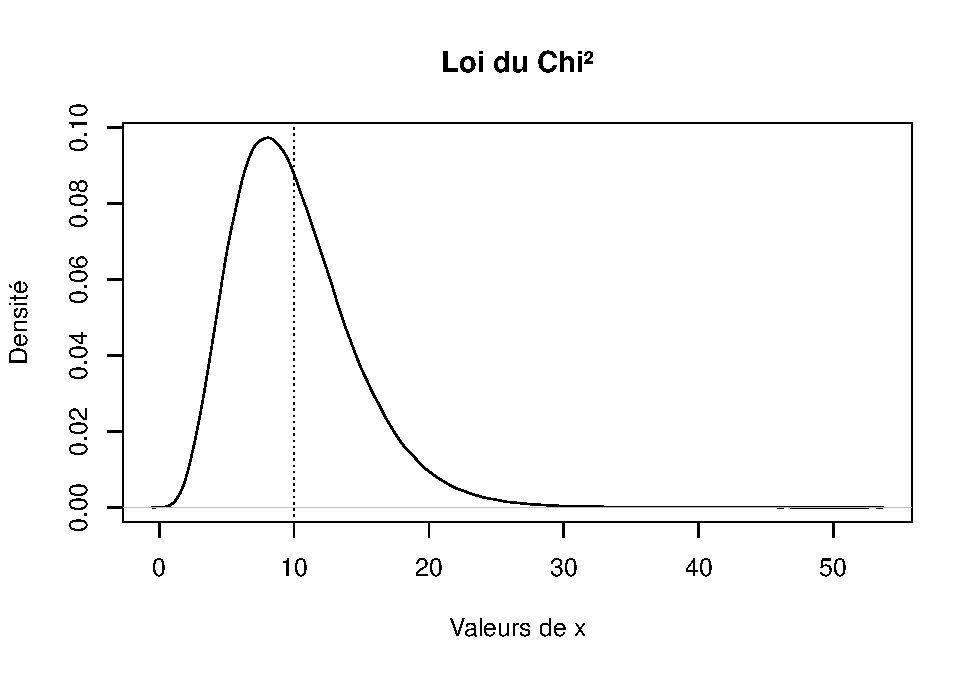
\includegraphics{_main_files/figure-latex/unnamed-chunk-7-1.pdf}
Dans des cas comme la loi normale, l'indicateur de position est centrale (ie. qu'il
y a une symétrie). Mais souvent, la répartition des poids n'est pas symétrique
et la moyenne est \emph{décalée} brisant la symétrie comme dans l'illustration
du Chi².

\hypertarget{autres-moyennes}{%
\subsection{Autres moyennes}\label{autres-moyennes}}

Elles sont peu utilisées.

\hypertarget{indicateur-de-dispersion}{%
\section{Indicateur de dispersion}\label{indicateur-de-dispersion}}

L'indicateur de dispersion le plus fréquent est l'écart-type. L'écart-type est
le carré des écarts à la moyenne (arithmétique).

Il vient naturellement avec la loi normale normale où 50\% des observations sont
à 1 écart-type autour de la moyenne.

Plus l'écart-type est grand plus les écarts entre les valeurs observées et la moyenne
sont grands. Les points sont plus dispersés.

\begin{Shaded}
\begin{Highlighting}[]
\NormalTok{y}\OtherTok{=}\FunctionTok{rnorm}\NormalTok{(}\DecValTok{1000000}\NormalTok{,}\DecValTok{1}\NormalTok{,}\DecValTok{1}\NormalTok{)}
\FunctionTok{plot}\NormalTok{(}\FunctionTok{density}\NormalTok{(y),}\AttributeTok{main=}\StringTok{"Normale de moyenne 1"}\NormalTok{,}\AttributeTok{xlab=}\StringTok{"Valeurs de x"}\NormalTok{,}\AttributeTok{ylab=}\StringTok{"Densité"}\NormalTok{)}
\FunctionTok{abline}\NormalTok{(}\AttributeTok{v=}\DecValTok{1}\NormalTok{,}\AttributeTok{lty=}\DecValTok{3}\NormalTok{)}
\FunctionTok{abline}\NormalTok{(}\AttributeTok{v=}\DecValTok{1}\SpecialCharTok{{-}}\FunctionTok{sd}\NormalTok{(y),}\AttributeTok{lty=}\DecValTok{1}\NormalTok{,}\AttributeTok{col=}\StringTok{"red"}\NormalTok{)}
\FunctionTok{abline}\NormalTok{(}\AttributeTok{v=}\DecValTok{1}\SpecialCharTok{+}\FunctionTok{sd}\NormalTok{(y),}\AttributeTok{lty=}\DecValTok{1}\NormalTok{,}\AttributeTok{col=}\StringTok{"red"}\NormalTok{)}
\FunctionTok{text}\NormalTok{(}\DecValTok{1}\SpecialCharTok{{-}}\FunctionTok{sd}\NormalTok{(y)}\SpecialCharTok{+}\FloatTok{0.5}\SpecialCharTok{*}\FunctionTok{sd}\NormalTok{(y),}\FloatTok{0.2}\SpecialCharTok{+}\FunctionTok{strheight}\NormalTok{(}\StringTok{"Ya"}\NormalTok{),}\FunctionTok{expression}\NormalTok{(sigma))}
\FunctionTok{text}\NormalTok{(}\DecValTok{1}\FloatTok{+0.5}\SpecialCharTok{*}\FunctionTok{sd}\NormalTok{(y),}\FloatTok{0.2}\SpecialCharTok{+}\FunctionTok{strheight}\NormalTok{(}\StringTok{"Ya"}\NormalTok{),}\FunctionTok{expression}\NormalTok{(sigma))}

\FunctionTok{arrows}\NormalTok{(}
  \DecValTok{1}\SpecialCharTok{{-}}\FunctionTok{sd}\NormalTok{(y),}\FloatTok{0.2}\SpecialCharTok{{-}}\FunctionTok{strheight}\NormalTok{(}\StringTok{"Ya"}\NormalTok{),}
  \DecValTok{1}\NormalTok{,}\FloatTok{0.2}\SpecialCharTok{{-}}\FunctionTok{strheight}\NormalTok{(}\StringTok{"Ya"}\NormalTok{),}
  \AttributeTok{length=}\FloatTok{0.05}\NormalTok{,}\AttributeTok{code=}\DecValTok{3}
\NormalTok{)}
\FunctionTok{arrows}\NormalTok{(}
  \DecValTok{1}\NormalTok{,}\FloatTok{0.2}\SpecialCharTok{{-}}\FunctionTok{strheight}\NormalTok{(}\StringTok{"Ya"}\NormalTok{),}
  \DecValTok{1}\SpecialCharTok{+}\FunctionTok{sd}\NormalTok{(y),}\FloatTok{0.2}\SpecialCharTok{{-}}\FunctionTok{strheight}\NormalTok{(}\StringTok{"Ya"}\NormalTok{),}
  \AttributeTok{length=}\FloatTok{0.05}\NormalTok{,}\AttributeTok{code=}\DecValTok{3}
\NormalTok{)}
\end{Highlighting}
\end{Shaded}

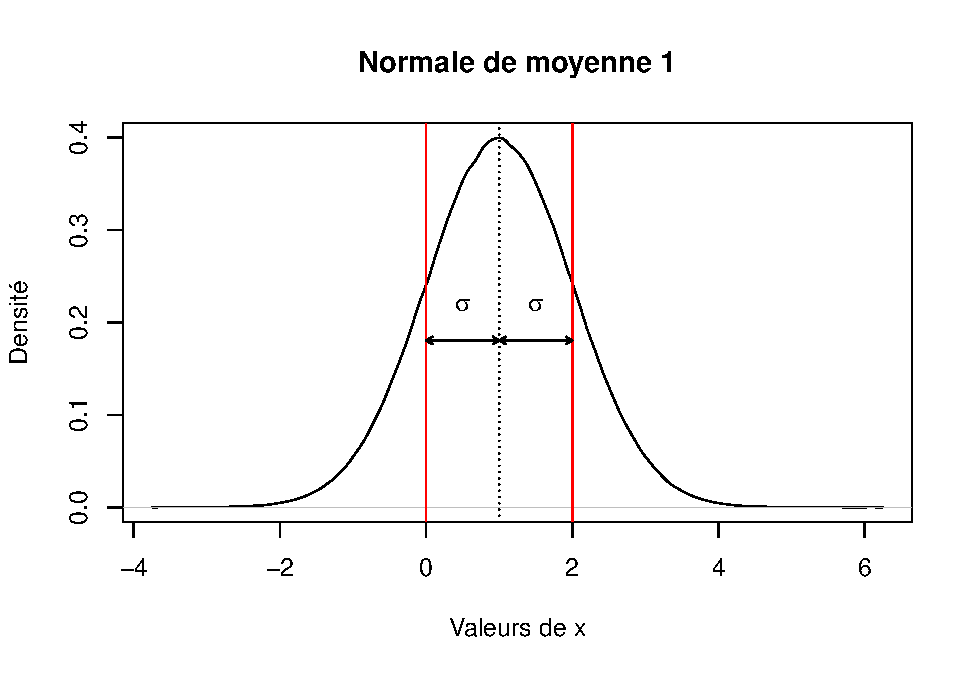
\includegraphics{_main_files/figure-latex/unnamed-chunk-8-1.pdf}
Un écart-type et la moyenne sont de même unité : par exemple si on mesure le poids
d'objets, on a par exemple moyenne et écart-type en \textbf{kg}.

Donc si on divise la moyenne par l'écart-type, on obtient un nombre sans unité ou
plutôt avec comme unité un écart-type. Ce type d'opération de diviser par l'écart-type
une ou des valeurs observées est appelé \textbf{réduire} une variable.

Cette opération est fréquemment associée au fait de soustraire par la moyenne avant
de réduire. Donc les observations deviennent \textbf{centrées} autour de la moyenne. On
appelle ces deux opérations centrer/réduire une variable soit \textbf{scale} en R.

Quand on analyse plusieurs variables d'unités très différentes en statistiques,
avec d'un côté des chiffres très grands et de l'autre côté des petits par
exemple, on est amené à centrer/réduire pour manipuler des chiffres de même
ordre de grandeur.

\hypertarget{les-indicateurs-de-la-loi-normale}{%
\section{Les indicateurs de la loi normale}\label{les-indicateurs-de-la-loi-normale}}

skweness et kurtosis.

La kurtose est l'aplatissement de la distribution par rapport à la loi normale.

\begin{Shaded}
\begin{Highlighting}[]
\NormalTok{rr }\OtherTok{\textless{}{-}} \FunctionTok{rnonnorm}\NormalTok{(}\DecValTok{1000000}\NormalTok{, }\AttributeTok{mean =} \DecValTok{0}\NormalTok{, }\AttributeTok{sd =} \DecValTok{1}\NormalTok{, }\AttributeTok{skew =} \DecValTok{0}\NormalTok{, }\AttributeTok{kurt =}  \DecValTok{0}\NormalTok{)}
\NormalTok{r2 }\OtherTok{\textless{}{-}} \FunctionTok{rnonnorm}\NormalTok{(}\DecValTok{1000000}\NormalTok{, }\AttributeTok{mean =} \DecValTok{0}\NormalTok{, }\AttributeTok{sd =} \DecValTok{1}\NormalTok{, }\AttributeTok{skew =} \DecValTok{0}\NormalTok{, }\AttributeTok{kurt =} \SpecialCharTok{{-}}\FloatTok{0.5}\NormalTok{)}
\NormalTok{r3 }\OtherTok{\textless{}{-}} \FunctionTok{rnonnorm}\NormalTok{(}\DecValTok{1000000}\NormalTok{, }\AttributeTok{mean =} \DecValTok{0}\NormalTok{, }\AttributeTok{sd =} \DecValTok{1}\NormalTok{, }\AttributeTok{skew =} \DecValTok{0}\NormalTok{, }\AttributeTok{kurt =}  \DecValTok{3}\NormalTok{)}

\NormalTok{d1 }\OtherTok{\textless{}{-}} \FunctionTok{density}\NormalTok{(rr}\SpecialCharTok{$}\NormalTok{dat)}
\NormalTok{d2 }\OtherTok{\textless{}{-}} \FunctionTok{density}\NormalTok{(r2}\SpecialCharTok{$}\NormalTok{dat)}
\NormalTok{d3 }\OtherTok{\textless{}{-}} \FunctionTok{density}\NormalTok{(r3}\SpecialCharTok{$}\NormalTok{dat)}

\FunctionTok{plot}\NormalTok{(}\DecValTok{0}\NormalTok{,}\DecValTok{0}\NormalTok{,}\AttributeTok{type=}\StringTok{"n"}\NormalTok{,}
     \AttributeTok{xlim=}\FunctionTok{range}\NormalTok{(}\FunctionTok{c}\NormalTok{(d1}\SpecialCharTok{$}\NormalTok{x,d2}\SpecialCharTok{$}\NormalTok{x,d3}\SpecialCharTok{$}\NormalTok{x)),}
     \AttributeTok{ylim=}\FunctionTok{range}\NormalTok{(}\FunctionTok{c}\NormalTok{(d1}\SpecialCharTok{$}\NormalTok{y,d2}\SpecialCharTok{$}\NormalTok{y,d3}\SpecialCharTok{$}\NormalTok{y)),}
     \AttributeTok{main =} \StringTok{""}\NormalTok{,}
     \AttributeTok{xlab=}\StringTok{"Valeurs"}\NormalTok{,}
     \AttributeTok{ylab=}\StringTok{"Densité"}
\NormalTok{       )}
\FunctionTok{lines}\NormalTok{(d1,}\AttributeTok{lty=}\DecValTok{1}\NormalTok{,}\AttributeTok{col=}\FunctionTok{brewer.pal}\NormalTok{(}\DecValTok{3}\NormalTok{,}\AttributeTok{name =} \StringTok{"Set2"}\NormalTok{)[}\DecValTok{1}\NormalTok{])}
\FunctionTok{lines}\NormalTok{(d2,}\AttributeTok{lty=}\DecValTok{2}\NormalTok{,}\AttributeTok{col=}\FunctionTok{brewer.pal}\NormalTok{(}\DecValTok{3}\NormalTok{,}\AttributeTok{name =} \StringTok{"Set2"}\NormalTok{)[}\DecValTok{2}\NormalTok{])}
\FunctionTok{lines}\NormalTok{(d3,}\AttributeTok{lty=}\DecValTok{3}\NormalTok{,}\AttributeTok{col=}\FunctionTok{brewer.pal}\NormalTok{(}\DecValTok{3}\NormalTok{,}\AttributeTok{name =} \StringTok{"Set2"}\NormalTok{)[}\DecValTok{3}\NormalTok{])}
\FunctionTok{legend}\NormalTok{(}\StringTok{"topright"}\NormalTok{,}\FunctionTok{c}\NormalTok{(}\StringTok{"Kurtose =    0"}\NormalTok{,}\StringTok{"Kurtose = {-}0.5"}\NormalTok{,}\StringTok{"Kurtose =  3"}\NormalTok{),}
       \AttributeTok{lty=}\FunctionTok{c}\NormalTok{(}\DecValTok{1}\NormalTok{,}\DecValTok{2}\NormalTok{,}\DecValTok{3}\NormalTok{),}
       \AttributeTok{col=}\FunctionTok{brewer.pal}\NormalTok{(}\DecValTok{3}\NormalTok{,}\AttributeTok{name =} \StringTok{"Set2"}\NormalTok{))}
\end{Highlighting}
\end{Shaded}

Le coefficient d'asymétrie ou skewness indique lui la symatrie par rapport à l'axe
centrale de la distribution normale.

\begin{Shaded}
\begin{Highlighting}[]
\NormalTok{rr }\OtherTok{\textless{}{-}} \FunctionTok{rnonnorm}\NormalTok{(}\DecValTok{9000000}\NormalTok{, }\AttributeTok{mean =} \DecValTok{0}\NormalTok{, }\AttributeTok{sd =} \DecValTok{1}\NormalTok{, }\AttributeTok{skew =}  \DecValTok{0}\NormalTok{  , }\AttributeTok{kurt =} \DecValTok{0}\NormalTok{)}
\NormalTok{r2 }\OtherTok{\textless{}{-}} \FunctionTok{rnonnorm}\NormalTok{(}\DecValTok{9000000}\NormalTok{, }\AttributeTok{mean =} \DecValTok{0}\NormalTok{, }\AttributeTok{sd =} \DecValTok{1}\NormalTok{, }\AttributeTok{skew =} \SpecialCharTok{{-}}\FloatTok{0.5}\NormalTok{, }\AttributeTok{kurt =} \DecValTok{0}\NormalTok{)}
\NormalTok{r3 }\OtherTok{\textless{}{-}} \FunctionTok{rnonnorm}\NormalTok{(}\DecValTok{9000000}\NormalTok{, }\AttributeTok{mean =} \DecValTok{0}\NormalTok{, }\AttributeTok{sd =} \DecValTok{1}\NormalTok{, }\AttributeTok{skew =}  \FloatTok{0.5}\NormalTok{, }\AttributeTok{kurt =} \DecValTok{0}\NormalTok{)}

\NormalTok{d1 }\OtherTok{\textless{}{-}} \FunctionTok{density}\NormalTok{(rr}\SpecialCharTok{$}\NormalTok{dat)}
\NormalTok{d2 }\OtherTok{\textless{}{-}} \FunctionTok{density}\NormalTok{(r2}\SpecialCharTok{$}\NormalTok{dat)}
\NormalTok{d3 }\OtherTok{\textless{}{-}} \FunctionTok{density}\NormalTok{(r3}\SpecialCharTok{$}\NormalTok{dat)}

\FunctionTok{plot}\NormalTok{(}\DecValTok{0}\NormalTok{,}\DecValTok{0}\NormalTok{,}\AttributeTok{type=}\StringTok{"n"}\NormalTok{,}
     \AttributeTok{xlim=}\FunctionTok{range}\NormalTok{(}\FunctionTok{c}\NormalTok{(d1}\SpecialCharTok{$}\NormalTok{x,d2}\SpecialCharTok{$}\NormalTok{x,d3}\SpecialCharTok{$}\NormalTok{x)),}
     \AttributeTok{ylim=}\FunctionTok{range}\NormalTok{(}\FunctionTok{c}\NormalTok{(d1}\SpecialCharTok{$}\NormalTok{y,d2}\SpecialCharTok{$}\NormalTok{y,d3}\SpecialCharTok{$}\NormalTok{y)),}
     \AttributeTok{main =} \StringTok{""}\NormalTok{,}
     \AttributeTok{xlab=}\StringTok{"Valeurs"}\NormalTok{,}
     \AttributeTok{ylab=}\StringTok{"Densité"}
\NormalTok{       )}
\FunctionTok{lines}\NormalTok{(d1,}\AttributeTok{lty=}\DecValTok{1}\NormalTok{,}\AttributeTok{col=}\FunctionTok{brewer.pal}\NormalTok{(}\DecValTok{3}\NormalTok{,}\AttributeTok{name =} \StringTok{"Set2"}\NormalTok{)[}\DecValTok{1}\NormalTok{])}
\FunctionTok{lines}\NormalTok{(d2,}\AttributeTok{lty=}\DecValTok{2}\NormalTok{,}\AttributeTok{col=}\FunctionTok{brewer.pal}\NormalTok{(}\DecValTok{3}\NormalTok{,}\AttributeTok{name =} \StringTok{"Set2"}\NormalTok{)[}\DecValTok{2}\NormalTok{])}
\FunctionTok{lines}\NormalTok{(d3,}\AttributeTok{lty=}\DecValTok{3}\NormalTok{,}\AttributeTok{col=}\FunctionTok{brewer.pal}\NormalTok{(}\DecValTok{3}\NormalTok{,}\AttributeTok{name =} \StringTok{"Set2"}\NormalTok{)[}\DecValTok{3}\NormalTok{])}
\FunctionTok{legend}\NormalTok{(}\StringTok{"topright"}\NormalTok{,}\FunctionTok{c}\NormalTok{(}\StringTok{"Skewness =    0"}\NormalTok{,}\StringTok{"Skewness = {-}0.5"}\NormalTok{,}\StringTok{"Skewness =  0.5"}\NormalTok{),}
       \AttributeTok{lty=}\FunctionTok{c}\NormalTok{(}\DecValTok{1}\NormalTok{,}\DecValTok{2}\NormalTok{,}\DecValTok{3}\NormalTok{),}
       \AttributeTok{col=}\FunctionTok{brewer.pal}\NormalTok{(}\DecValTok{3}\NormalTok{,}\AttributeTok{name =} \StringTok{"Set2"}\NormalTok{))}
\end{Highlighting}
\end{Shaded}

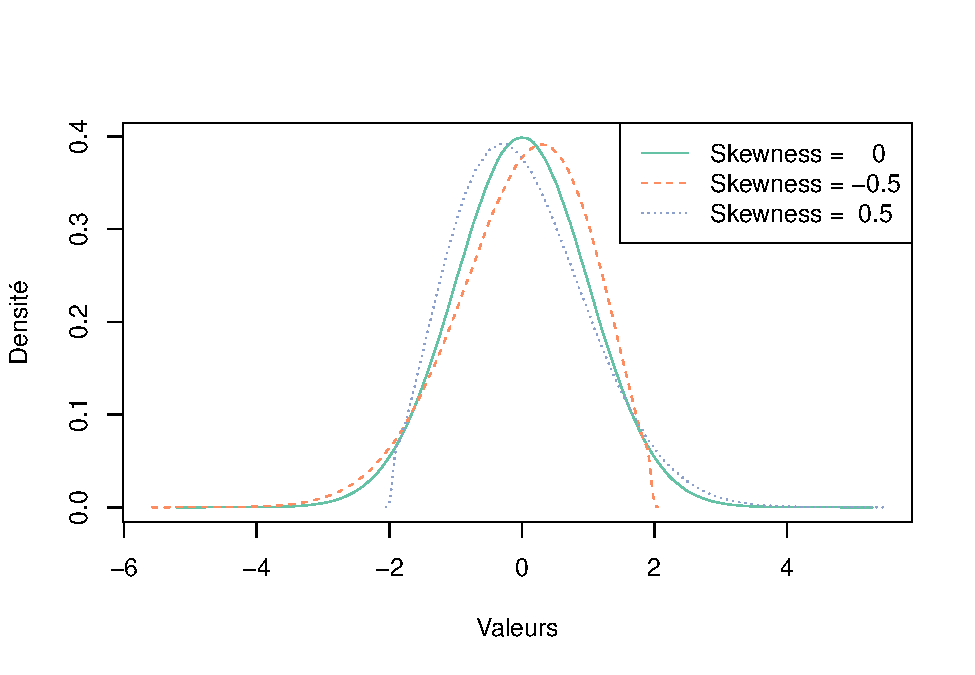
\includegraphics{_main_files/figure-latex/unnamed-chunk-10-1.pdf}

\hypertarget{quantiles-ex-de-la-loi-normale.}{%
\section{Quantiles, ex de la loi normale.}\label{quantiles-ex-de-la-loi-normale.}}

Les quantiles représentent la proportion d'individus qui se retrouvent en deça
d'une valeur. Par exemple, pour une loi normale :

\begin{Shaded}
\begin{Highlighting}[]
\NormalTok{rr }\OtherTok{\textless{}{-}} \FunctionTok{rnorm}\NormalTok{(}\DecValTok{1000000}\NormalTok{)}
\NormalTok{dd }\OtherTok{\textless{}{-}} \FunctionTok{density}\NormalTok{(rr)}

\FunctionTok{plot}\NormalTok{(}\DecValTok{0}\NormalTok{,}\DecValTok{0}\NormalTok{,}\AttributeTok{type=}\StringTok{"n"}\NormalTok{,}\AttributeTok{main=}\StringTok{""}\NormalTok{,}\AttributeTok{xlab=}\StringTok{"Valeurs"}\NormalTok{,}\AttributeTok{ylab=}\StringTok{"Densité"}\NormalTok{,}
     \AttributeTok{xlim=}\FunctionTok{range}\NormalTok{(dd}\SpecialCharTok{$}\NormalTok{x),}\AttributeTok{ylim=}\FunctionTok{range}\NormalTok{(dd}\SpecialCharTok{$}\NormalTok{y))}
\FunctionTok{lines}\NormalTok{(dd)}
\FunctionTok{polygon}\NormalTok{(}\FunctionTok{c}\NormalTok{(dd}\SpecialCharTok{$}\NormalTok{x[dd}\SpecialCharTok{$}\NormalTok{x }\SpecialCharTok{\textless{}} \SpecialCharTok{{-}}\DecValTok{1}\NormalTok{],}\FunctionTok{rev}\NormalTok{(dd}\SpecialCharTok{$}\NormalTok{x[dd}\SpecialCharTok{$}\NormalTok{x }\SpecialCharTok{\textless{}} \SpecialCharTok{{-}}\DecValTok{1}\NormalTok{])),}
        \FunctionTok{c}\NormalTok{(dd}\SpecialCharTok{$}\NormalTok{y[dd}\SpecialCharTok{$}\NormalTok{x }\SpecialCharTok{\textless{}} \SpecialCharTok{{-}}\DecValTok{1}\NormalTok{],}\FunctionTok{rep}\NormalTok{(}\DecValTok{0}\NormalTok{,}\FunctionTok{length}\NormalTok{(dd}\SpecialCharTok{$}\NormalTok{y))[dd}\SpecialCharTok{$}\NormalTok{x }\SpecialCharTok{\textless{}} \SpecialCharTok{{-}}\DecValTok{1}\NormalTok{]),}
        \AttributeTok{col=}\FunctionTok{rgb}\NormalTok{(}\DecValTok{0}\NormalTok{,}\DecValTok{0}\NormalTok{,}\DecValTok{1}\NormalTok{,}\FloatTok{0.5}\NormalTok{),}\AttributeTok{border =} \ConstantTok{NA}\NormalTok{)}
\FunctionTok{abline}\NormalTok{(}\AttributeTok{v=}\SpecialCharTok{{-}}\DecValTok{1}\NormalTok{)}
\FunctionTok{text}\NormalTok{(}\SpecialCharTok{{-}}\DecValTok{3}\NormalTok{,}\FloatTok{0.3}\NormalTok{,}\FunctionTok{paste}\NormalTok{(}\FunctionTok{round}\NormalTok{(}\DecValTok{100}\SpecialCharTok{*}\FunctionTok{pnorm}\NormalTok{(}\SpecialCharTok{{-}}\DecValTok{1}\NormalTok{),}\DecValTok{2}\NormalTok{),}\StringTok{" \% en deça de "}\NormalTok{,}\FunctionTok{round}\NormalTok{(}\SpecialCharTok{{-}}\DecValTok{1}\NormalTok{,}\DecValTok{2}\NormalTok{)))}
\end{Highlighting}
\end{Shaded}

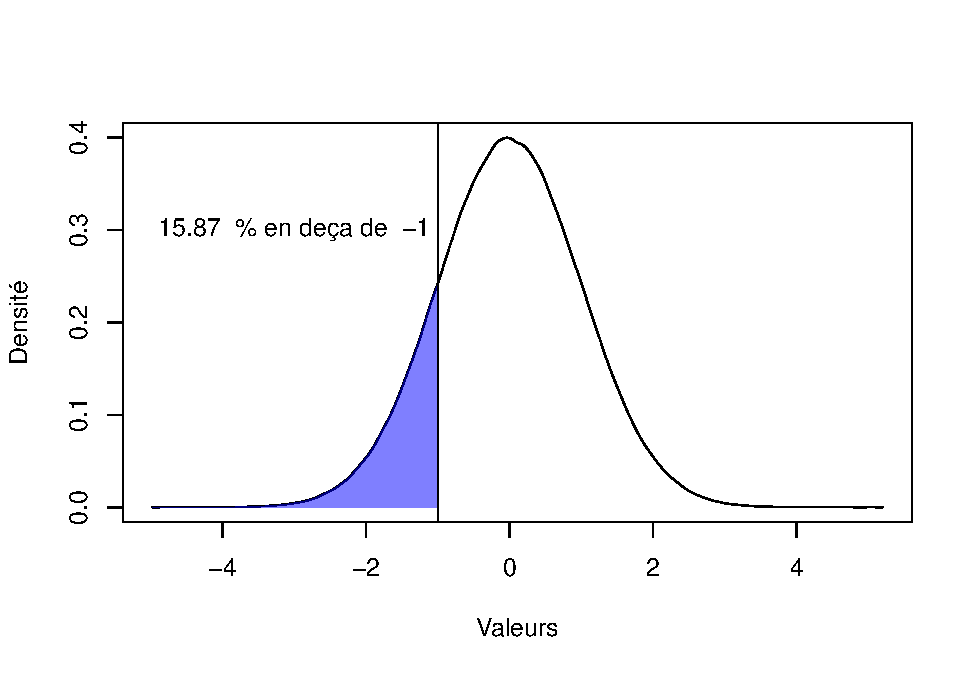
\includegraphics{_main_files/figure-latex/unnamed-chunk-11-1.pdf}

\begin{Shaded}
\begin{Highlighting}[]
\FunctionTok{plot}\NormalTok{(}\DecValTok{0}\NormalTok{,}\DecValTok{0}\NormalTok{,}\AttributeTok{type=}\StringTok{"n"}\NormalTok{,}\AttributeTok{main=}\StringTok{""}\NormalTok{,}\AttributeTok{xlab=}\StringTok{"Valeurs"}\NormalTok{,}\AttributeTok{ylab=}\StringTok{"Densité"}\NormalTok{,}
     \AttributeTok{xlim=}\FunctionTok{range}\NormalTok{(dd}\SpecialCharTok{$}\NormalTok{x),}\AttributeTok{ylim=}\FunctionTok{range}\NormalTok{(dd}\SpecialCharTok{$}\NormalTok{y))}
\FunctionTok{lines}\NormalTok{(dd)}
\FunctionTok{polygon}\NormalTok{(}\FunctionTok{c}\NormalTok{(dd}\SpecialCharTok{$}\NormalTok{x[dd}\SpecialCharTok{$}\NormalTok{x }\SpecialCharTok{\textless{}} \DecValTok{1}\NormalTok{],}\FunctionTok{rev}\NormalTok{(dd}\SpecialCharTok{$}\NormalTok{x[dd}\SpecialCharTok{$}\NormalTok{x }\SpecialCharTok{\textless{}} \DecValTok{1}\NormalTok{])),}
        \FunctionTok{c}\NormalTok{(dd}\SpecialCharTok{$}\NormalTok{y[dd}\SpecialCharTok{$}\NormalTok{x }\SpecialCharTok{\textless{}} \DecValTok{1}\NormalTok{],}\FunctionTok{rep}\NormalTok{(}\DecValTok{0}\NormalTok{,}\FunctionTok{length}\NormalTok{(dd}\SpecialCharTok{$}\NormalTok{y))[dd}\SpecialCharTok{$}\NormalTok{x }\SpecialCharTok{\textless{}} \DecValTok{1}\NormalTok{]),}
        \AttributeTok{col=}\FunctionTok{rgb}\NormalTok{(}\DecValTok{0}\NormalTok{,}\DecValTok{1}\NormalTok{,}\DecValTok{0}\NormalTok{,}\FloatTok{0.5}\NormalTok{),}\AttributeTok{border =} \ConstantTok{NA}\NormalTok{)}
\FunctionTok{abline}\NormalTok{(}\AttributeTok{v=}\DecValTok{1}\NormalTok{)}
\FunctionTok{text}\NormalTok{(}\SpecialCharTok{{-}}\DecValTok{3}\NormalTok{,}\FloatTok{0.3}\NormalTok{,}\FunctionTok{paste}\NormalTok{(}\FunctionTok{round}\NormalTok{(}\DecValTok{100}\SpecialCharTok{*}\FunctionTok{pnorm}\NormalTok{(}\DecValTok{1}\NormalTok{),}\DecValTok{2}\NormalTok{),}\StringTok{" \% en deça de "}\NormalTok{,}\FunctionTok{round}\NormalTok{(}\DecValTok{1}\NormalTok{,}\DecValTok{2}\NormalTok{)))}
\end{Highlighting}
\end{Shaded}

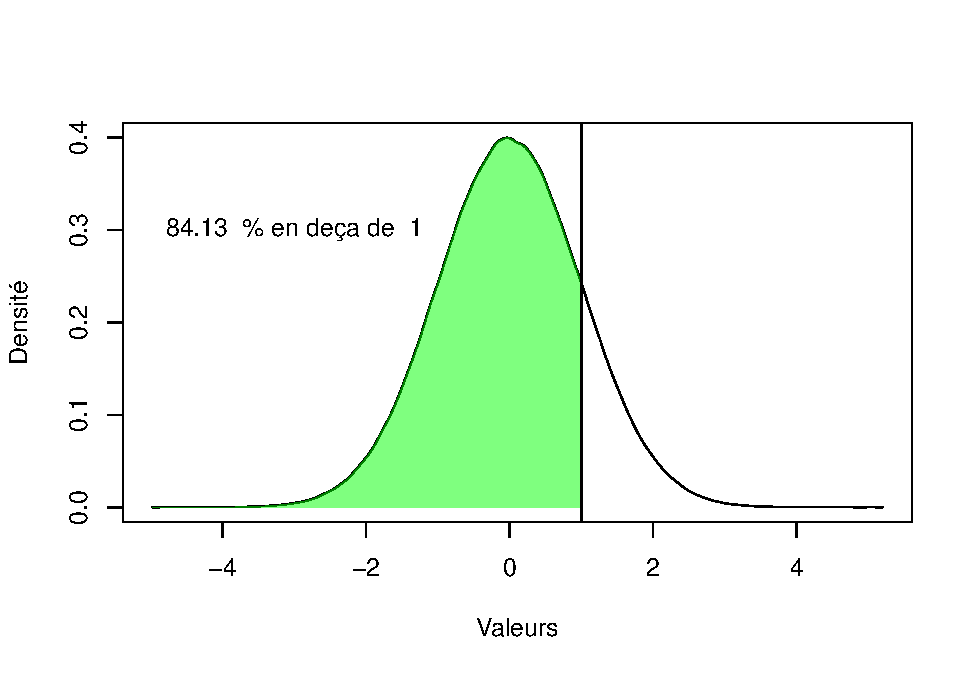
\includegraphics{_main_files/figure-latex/unnamed-chunk-12-1.pdf}

\begin{Shaded}
\begin{Highlighting}[]
\FunctionTok{plot}\NormalTok{(}\DecValTok{0}\NormalTok{,}\DecValTok{0}\NormalTok{,}\AttributeTok{type=}\StringTok{"n"}\NormalTok{,}\AttributeTok{main=}\StringTok{""}\NormalTok{,}\AttributeTok{xlab=}\StringTok{"Valeurs"}\NormalTok{,}\AttributeTok{ylab=}\StringTok{"Densité"}\NormalTok{,}
     \AttributeTok{xlim=}\FunctionTok{range}\NormalTok{(dd}\SpecialCharTok{$}\NormalTok{x),}\AttributeTok{ylim=}\FunctionTok{range}\NormalTok{(dd}\SpecialCharTok{$}\NormalTok{y))}
\FunctionTok{lines}\NormalTok{(dd)}
\FunctionTok{polygon}\NormalTok{(}\FunctionTok{c}\NormalTok{(dd}\SpecialCharTok{$}\NormalTok{x[dd}\SpecialCharTok{$}\NormalTok{x }\SpecialCharTok{\textless{}} \DecValTok{1}\NormalTok{],}\FunctionTok{rev}\NormalTok{(dd}\SpecialCharTok{$}\NormalTok{x[dd}\SpecialCharTok{$}\NormalTok{x }\SpecialCharTok{\textless{}} \DecValTok{1}\NormalTok{])),}
        \FunctionTok{c}\NormalTok{(dd}\SpecialCharTok{$}\NormalTok{y[dd}\SpecialCharTok{$}\NormalTok{x }\SpecialCharTok{\textless{}} \DecValTok{1}\NormalTok{],}\FunctionTok{rep}\NormalTok{(}\DecValTok{0}\NormalTok{,}\FunctionTok{length}\NormalTok{(dd}\SpecialCharTok{$}\NormalTok{y))[dd}\SpecialCharTok{$}\NormalTok{x }\SpecialCharTok{\textless{}} \DecValTok{1}\NormalTok{]),}
        \AttributeTok{col=}\FunctionTok{rgb}\NormalTok{(}\DecValTok{0}\NormalTok{,}\DecValTok{1}\NormalTok{,}\DecValTok{0}\NormalTok{,}\FloatTok{0.5}\NormalTok{),}\AttributeTok{border =} \ConstantTok{NA}\NormalTok{)}
\FunctionTok{abline}\NormalTok{(}\AttributeTok{v=}\DecValTok{1}\NormalTok{)}
\FunctionTok{text}\NormalTok{(}\SpecialCharTok{{-}}\DecValTok{3}\NormalTok{,}\FloatTok{0.3}\NormalTok{,}\FunctionTok{paste}\NormalTok{(}\DecValTok{100}\SpecialCharTok{*}\FunctionTok{round}\NormalTok{(}\FunctionTok{pnorm}\NormalTok{(}\DecValTok{1}\NormalTok{),}\DecValTok{2}\NormalTok{),}\StringTok{" \% en deça de "}\NormalTok{,}\FunctionTok{round}\NormalTok{(}\DecValTok{1}\NormalTok{,}\DecValTok{2}\NormalTok{)))}
\end{Highlighting}
\end{Shaded}

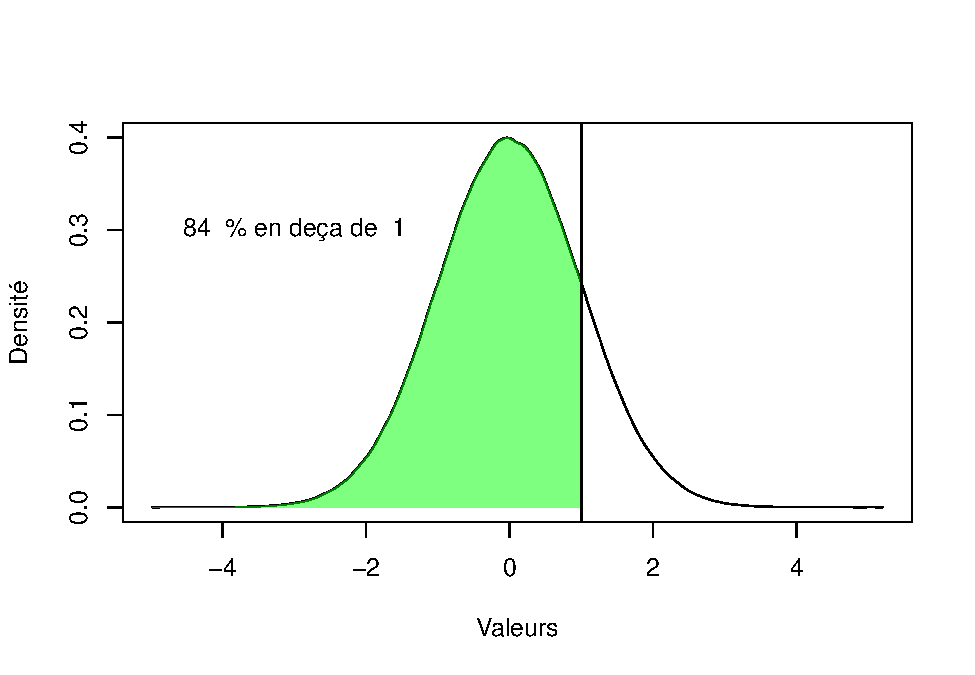
\includegraphics{_main_files/figure-latex/unnamed-chunk-13-1.pdf}

Soit entre la moyenne et les écart-types pour la loi normale, il y a
68 \% des individus.

\begin{Shaded}
\begin{Highlighting}[]
\FunctionTok{plot}\NormalTok{(}\DecValTok{0}\NormalTok{,}\DecValTok{0}\NormalTok{,}\AttributeTok{type=}\StringTok{"n"}\NormalTok{,}\AttributeTok{main=}\StringTok{""}\NormalTok{,}\AttributeTok{xlab=}\StringTok{"Valeurs"}\NormalTok{,}\AttributeTok{ylab=}\StringTok{"Densité"}\NormalTok{,}
     \AttributeTok{xlim=}\FunctionTok{range}\NormalTok{(dd}\SpecialCharTok{$}\NormalTok{x),}\AttributeTok{ylim=}\FunctionTok{range}\NormalTok{(dd}\SpecialCharTok{$}\NormalTok{y))}
\FunctionTok{lines}\NormalTok{(dd)}
\FunctionTok{polygon}\NormalTok{(}\FunctionTok{c}\NormalTok{(dd}\SpecialCharTok{$}\NormalTok{x[dd}\SpecialCharTok{$}\NormalTok{x }\SpecialCharTok{\textgreater{}} \SpecialCharTok{{-}}\DecValTok{1} \SpecialCharTok{\&}\NormalTok{ dd}\SpecialCharTok{$}\NormalTok{x }\SpecialCharTok{\textless{}} \DecValTok{1}\NormalTok{],}\FunctionTok{rev}\NormalTok{(dd}\SpecialCharTok{$}\NormalTok{x[dd}\SpecialCharTok{$}\NormalTok{x }\SpecialCharTok{\textgreater{}} \SpecialCharTok{{-}}\DecValTok{1} \SpecialCharTok{\&}\NormalTok{ dd}\SpecialCharTok{$}\NormalTok{x }\SpecialCharTok{\textless{}} \DecValTok{1}\NormalTok{])),}
        \FunctionTok{c}\NormalTok{(dd}\SpecialCharTok{$}\NormalTok{y[dd}\SpecialCharTok{$}\NormalTok{x }\SpecialCharTok{\textgreater{}} \SpecialCharTok{{-}}\DecValTok{1} \SpecialCharTok{\&}\NormalTok{ dd}\SpecialCharTok{$}\NormalTok{x }\SpecialCharTok{\textless{}} \DecValTok{1}\NormalTok{],}\FunctionTok{rep}\NormalTok{(}\DecValTok{0}\NormalTok{,}\FunctionTok{length}\NormalTok{(dd}\SpecialCharTok{$}\NormalTok{y))[dd}\SpecialCharTok{$}\NormalTok{x }\SpecialCharTok{\textgreater{}} \SpecialCharTok{{-}}\DecValTok{1} \SpecialCharTok{\&}\NormalTok{ dd}\SpecialCharTok{$}\NormalTok{x }\SpecialCharTok{\textless{}} \DecValTok{1}\NormalTok{]),}
        \AttributeTok{col=}\FunctionTok{rgb}\NormalTok{(}\DecValTok{0}\NormalTok{,}\DecValTok{1}\NormalTok{,}\DecValTok{0}\NormalTok{,}\FloatTok{0.5}\NormalTok{),}\AttributeTok{border =} \ConstantTok{NA}\NormalTok{)}
\FunctionTok{abline}\NormalTok{(}\AttributeTok{v=}\SpecialCharTok{{-}}\DecValTok{1}\NormalTok{,}\AttributeTok{lty=}\DecValTok{3}\NormalTok{)}
\FunctionTok{abline}\NormalTok{(}\AttributeTok{v=} \DecValTok{1}\NormalTok{,}\AttributeTok{lty=}\DecValTok{3}\NormalTok{)}
\FunctionTok{text}\NormalTok{(}\SpecialCharTok{{-}}\DecValTok{3}\NormalTok{,}\FloatTok{0.3}\NormalTok{,}\FunctionTok{paste}\NormalTok{(}\DecValTok{100}\SpecialCharTok{*}\FunctionTok{round}\NormalTok{(}\FunctionTok{pnorm}\NormalTok{(}\DecValTok{1}\NormalTok{) }\SpecialCharTok{{-}} \FunctionTok{pnorm}\NormalTok{(}\SpecialCharTok{{-}}\DecValTok{1}\NormalTok{),}\DecValTok{2}\NormalTok{),}\StringTok{" \% entre {-}1 et 1"}\NormalTok{))}
\end{Highlighting}
\end{Shaded}

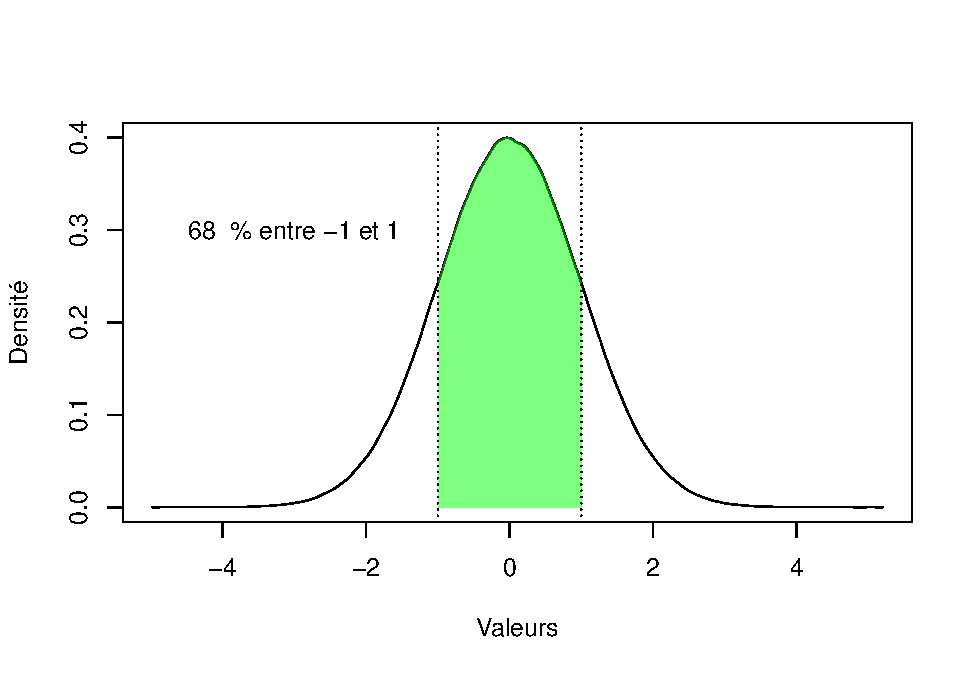
\includegraphics{_main_files/figure-latex/unnamed-chunk-14-1.pdf}

Entre les valeurs, les quantiles -2 et 2, il y a
95 \% des individus.

Les valeurs pour -2 et 2 sont respectivement -1,96 et 1,96.

\hypertarget{la-muxe9diane-et-les-quantiles-usuelles}{%
\section{La médiane et les quantiles usuelles}\label{la-muxe9diane-et-les-quantiles-usuelles}}

La médiane est le quantile le plus connu : il sépare 50\% des individus à gauche
et 50 \% des individus à droite. Quand la fonction est symétrique, la médiane est
égale à la moyenne.

La médiane est souvent utilisé comme indicatrice de tendance centrale dans le
cas où la fonction est très asymétrique où s'il y a des valeurs extrêmes :

\begin{Shaded}
\begin{Highlighting}[]
\NormalTok{rr }\OtherTok{\textless{}{-}} \FunctionTok{c}\NormalTok{(}\FunctionTok{rnorm}\NormalTok{(}\DecValTok{1000}\NormalTok{),}\FunctionTok{rnorm}\NormalTok{(}\DecValTok{5}\NormalTok{,}\DecValTok{10}\NormalTok{))}
\FunctionTok{plot}\NormalTok{(}\FunctionTok{density}\NormalTok{(rr))}
\end{Highlighting}
\end{Shaded}

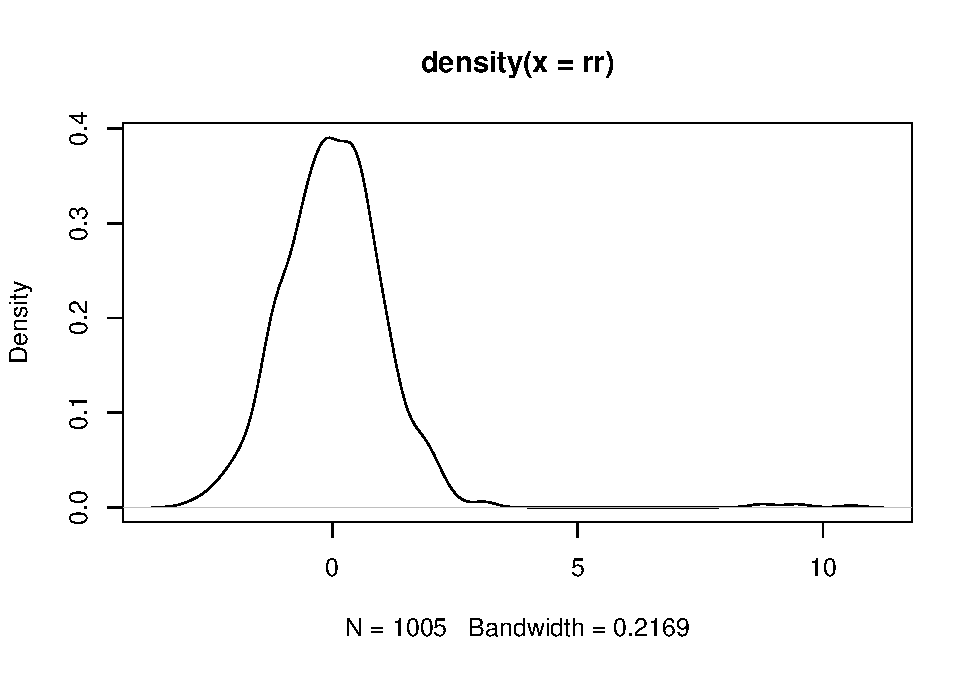
\includegraphics{_main_files/figure-latex/unnamed-chunk-15-1.pdf}
la moyenne est de 0.0364018 et l'écart-type de 1.181116. La moyenne sans
les points extrêmes est de -0.0104208 tandis que la médiane est de
-0.007937 avec et de -0.0146233.

Les autres quantiles quantiles les plus fréquents sont les quartiles :
0\%, 25\%, 50\%, 75\%, 100\%.

\hypertarget{corruxe9lations}{%
\section{Corrélations}\label{corruxe9lations}}

\begin{Shaded}
\begin{Highlighting}[]
\FunctionTok{set.seed}\NormalTok{(}\DecValTok{42}\NormalTok{)}
\NormalTok{rx }\OtherTok{\textless{}{-}} \FunctionTok{runif}\NormalTok{(}\DecValTok{100}\NormalTok{,}\DecValTok{0}\NormalTok{,}\DecValTok{4}\NormalTok{)}
\NormalTok{ry }\OtherTok{\textless{}{-}} \FloatTok{0.8}\SpecialCharTok{*}\NormalTok{rx}\SpecialCharTok{+}\FunctionTok{rnorm}\NormalTok{(}\DecValTok{100}\NormalTok{,}\AttributeTok{sd=}\FloatTok{0.5}\NormalTok{)}
\FunctionTok{plot}\NormalTok{(rx,ry,}\AttributeTok{pch=}\DecValTok{20}\NormalTok{)}
\end{Highlighting}
\end{Shaded}

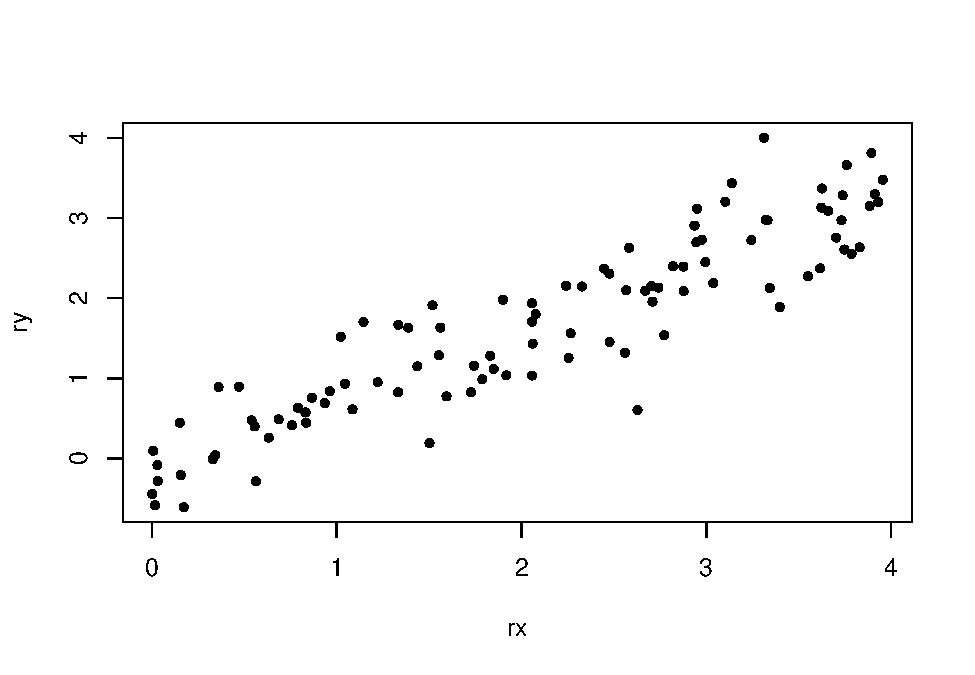
\includegraphics{_main_files/figure-latex/unnamed-chunk-16-1.pdf}

\begin{Shaded}
\begin{Highlighting}[]
\FunctionTok{set.seed}\NormalTok{(}\DecValTok{42}\NormalTok{)}
\NormalTok{rx }\OtherTok{\textless{}{-}} \FunctionTok{runif}\NormalTok{(}\DecValTok{100}\NormalTok{,}\DecValTok{0}\NormalTok{,}\DecValTok{4}\NormalTok{)}
\NormalTok{ry }\OtherTok{\textless{}{-}} \FloatTok{0.8}\SpecialCharTok{*}\NormalTok{rx}\SpecialCharTok{+}\FunctionTok{rnorm}\NormalTok{(}\DecValTok{100}\NormalTok{,}\AttributeTok{sd=}\FloatTok{0.5}\NormalTok{)}
\FunctionTok{plot}\NormalTok{(rx,ry,}\AttributeTok{pch=}\DecValTok{20}\NormalTok{)}
\NormalTok{rr }\OtherTok{\textless{}{-}} \FunctionTok{lm}\NormalTok{(ry}\SpecialCharTok{\textasciitilde{}}\NormalTok{rx)}
\FunctionTok{abline}\NormalTok{(rr)}
\NormalTok{pos }\OtherTok{\textless{}{-}} \FunctionTok{which.max}\NormalTok{(ry)}
  \FunctionTok{arrows}\NormalTok{(rx[pos],}\FunctionTok{predict}\NormalTok{(rr)[pos],rx[pos],ry[pos],}\AttributeTok{length=}\FloatTok{0.05}\NormalTok{,}\AttributeTok{code =} \DecValTok{3}\NormalTok{)}
\end{Highlighting}
\end{Shaded}

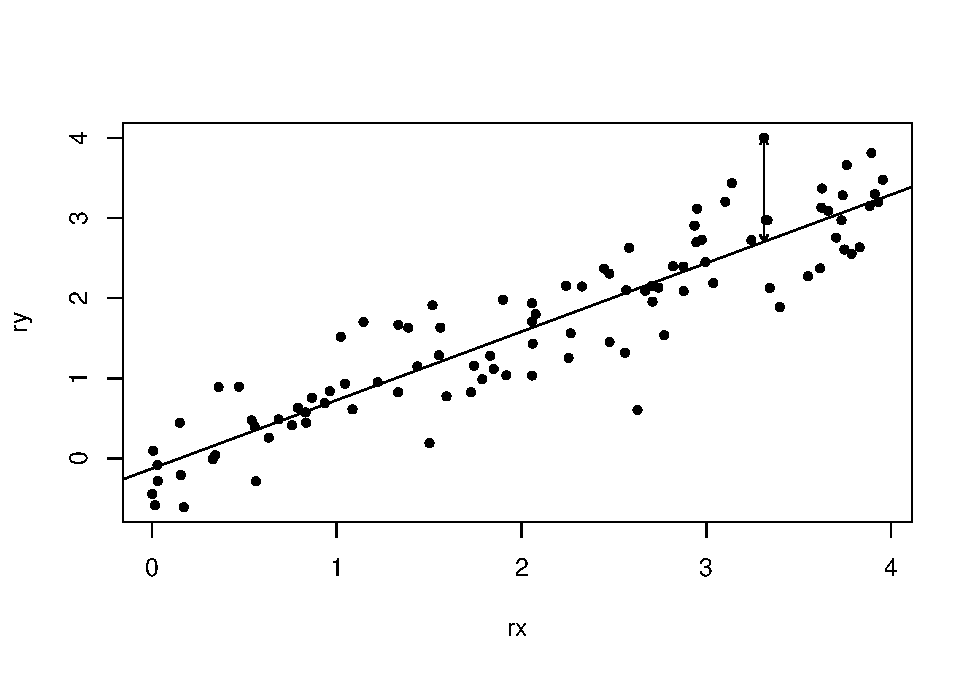
\includegraphics{_main_files/figure-latex/unnamed-chunk-17-1.pdf}

\begin{Shaded}
\begin{Highlighting}[]
\FunctionTok{print}\NormalTok{(rr)}
\end{Highlighting}
\end{Shaded}

\begin{verbatim}
## 
## Call:
## lm(formula = ry ~ rx)
## 
## Coefficients:
## (Intercept)           rx  
##     -0.1269       0.8545
\end{verbatim}

\begin{Shaded}
\begin{Highlighting}[]
\FunctionTok{set.seed}\NormalTok{(}\DecValTok{42}\NormalTok{)}
\NormalTok{rx }\OtherTok{\textless{}{-}} \FunctionTok{runif}\NormalTok{(}\DecValTok{100}\NormalTok{,}\SpecialCharTok{{-}}\DecValTok{4}\NormalTok{,}\DecValTok{4}\NormalTok{)}
\NormalTok{ry }\OtherTok{\textless{}{-}} \FunctionTok{runif}\NormalTok{(}\DecValTok{100}\NormalTok{,}\SpecialCharTok{{-}}\DecValTok{4}\NormalTok{,}\DecValTok{4}\NormalTok{)}
\FunctionTok{plot}\NormalTok{(rx,ry,}\AttributeTok{pch=}\DecValTok{20}\NormalTok{)}
\NormalTok{rr }\OtherTok{\textless{}{-}} \FunctionTok{lm}\NormalTok{(ry}\SpecialCharTok{\textasciitilde{}}\NormalTok{rx)}
\FunctionTok{abline}\NormalTok{(rr)}
\end{Highlighting}
\end{Shaded}

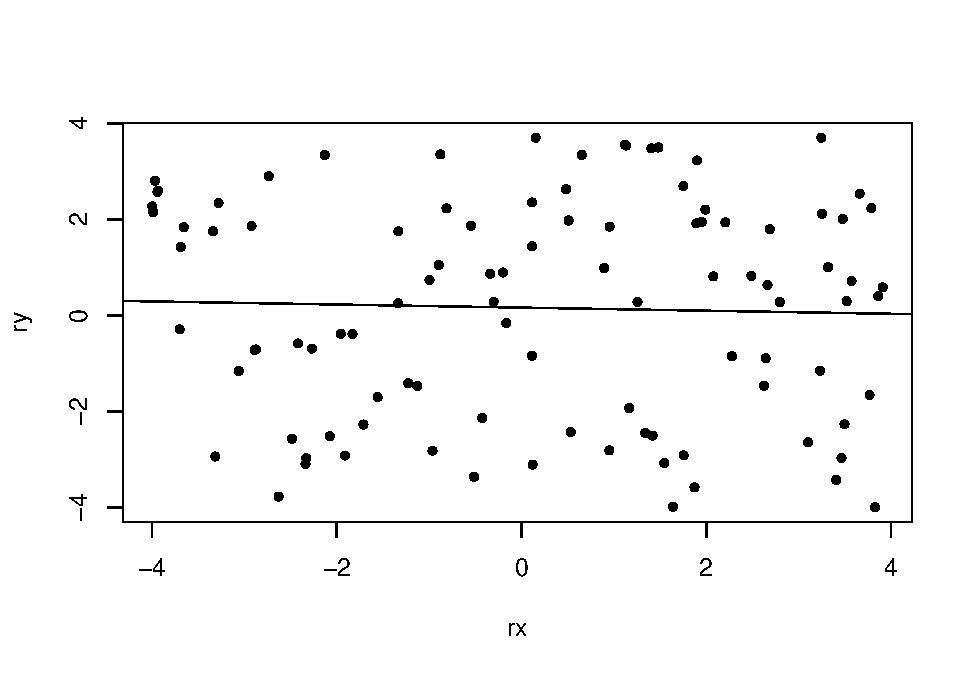
\includegraphics{_main_files/figure-latex/unnamed-chunk-19-1.pdf}

\begin{Shaded}
\begin{Highlighting}[]
\FunctionTok{set.seed}\NormalTok{(}\DecValTok{42}\NormalTok{)}
\NormalTok{rx }\OtherTok{\textless{}{-}} \FunctionTok{runif}\NormalTok{(}\DecValTok{100}\NormalTok{,}\SpecialCharTok{{-}}\DecValTok{4}\NormalTok{,}\DecValTok{4}\NormalTok{)}
\NormalTok{ry }\OtherTok{\textless{}{-}} \FunctionTok{cos}\NormalTok{(rx)}\SpecialCharTok{+}\FunctionTok{rnorm}\NormalTok{(}\DecValTok{100}\NormalTok{,}\AttributeTok{sd=}\FloatTok{0.25}\NormalTok{)}
\FunctionTok{plot}\NormalTok{(rx,ry,}\AttributeTok{pch=}\DecValTok{20}\NormalTok{)}
\NormalTok{rr }\OtherTok{\textless{}{-}} \FunctionTok{lm}\NormalTok{(ry}\SpecialCharTok{\textasciitilde{}}\NormalTok{rx)}
\FunctionTok{abline}\NormalTok{(rr)}
\end{Highlighting}
\end{Shaded}

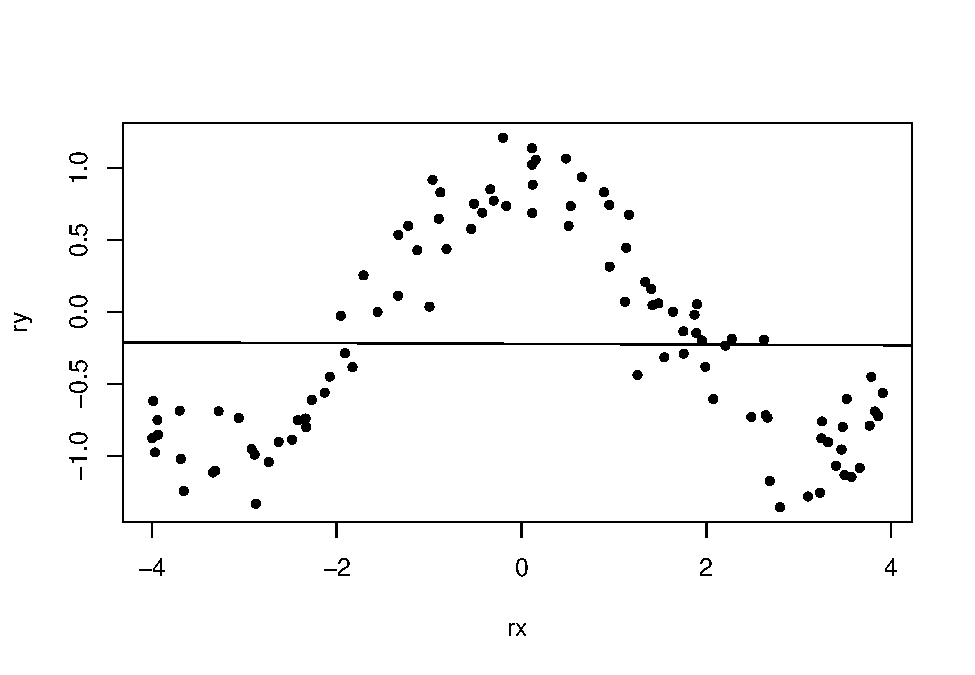
\includegraphics{_main_files/figure-latex/unnamed-chunk-20-1.pdf}

\begin{Shaded}
\begin{Highlighting}[]
\FunctionTok{print}\NormalTok{(rr)}
\end{Highlighting}
\end{Shaded}

\begin{verbatim}
## 
## Call:
## lm(formula = ry ~ rx)
## 
## Coefficients:
## (Intercept)           rx  
##   -0.221598    -0.002439
\end{verbatim}

\begin{Shaded}
\begin{Highlighting}[]
\FunctionTok{set.seed}\NormalTok{(}\DecValTok{42}\NormalTok{)}
\NormalTok{rx }\OtherTok{\textless{}{-}} \FunctionTok{runif}\NormalTok{(}\DecValTok{100}\NormalTok{,}\SpecialCharTok{{-}}\DecValTok{4}\NormalTok{,}\DecValTok{4}\NormalTok{)}
\NormalTok{ry }\OtherTok{\textless{}{-}}\NormalTok{ rx}\SpecialCharTok{\^{}}\DecValTok{2}\SpecialCharTok{+}\FunctionTok{rnorm}\NormalTok{(}\DecValTok{100}\NormalTok{,}\AttributeTok{sd=}\DecValTok{1}\NormalTok{)}
\FunctionTok{plot}\NormalTok{(rx,ry,}\AttributeTok{pch=}\DecValTok{20}\NormalTok{)}
\NormalTok{rr }\OtherTok{\textless{}{-}} \FunctionTok{lm}\NormalTok{(ry}\SpecialCharTok{\textasciitilde{}}\NormalTok{rx)}
\FunctionTok{abline}\NormalTok{(rr)}
\end{Highlighting}
\end{Shaded}

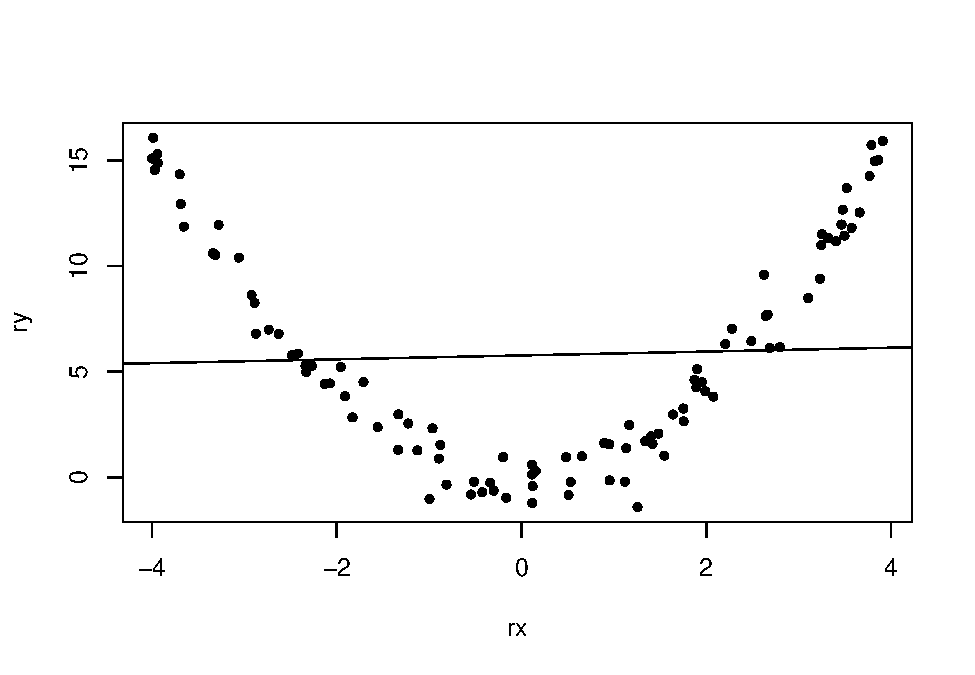
\includegraphics{_main_files/figure-latex/unnamed-chunk-22-1.pdf}

\begin{Shaded}
\begin{Highlighting}[]
\NormalTok{rr}
\end{Highlighting}
\end{Shaded}

\begin{verbatim}
## 
## Call:
## lm(formula = ry ~ rx)
## 
## Coefficients:
## (Intercept)           rx  
##     5.77183      0.09141
\end{verbatim}

\begin{Shaded}
\begin{Highlighting}[]
\NormalTok{a }\OtherTok{\textless{}{-}} \FunctionTok{lm}\NormalTok{(ry }\SpecialCharTok{\textasciitilde{}}\NormalTok{ rx }\SpecialCharTok{+} \FunctionTok{I}\NormalTok{(rx}\SpecialCharTok{\^{}}\DecValTok{2}\NormalTok{))}
\FunctionTok{plot}\NormalTok{(rx,ry,}\AttributeTok{pch=}\DecValTok{20}\NormalTok{)}
\FunctionTok{points}\NormalTok{(rx[}\FunctionTok{order}\NormalTok{(rx)],}\FunctionTok{predict}\NormalTok{(a)[}\FunctionTok{order}\NormalTok{(rx)],}\AttributeTok{col=}\FunctionTok{rgb}\NormalTok{(}\DecValTok{0}\NormalTok{,}\DecValTok{0}\NormalTok{,}\DecValTok{1}\NormalTok{),}\AttributeTok{type=}\StringTok{"l"}\NormalTok{)}
\end{Highlighting}
\end{Shaded}

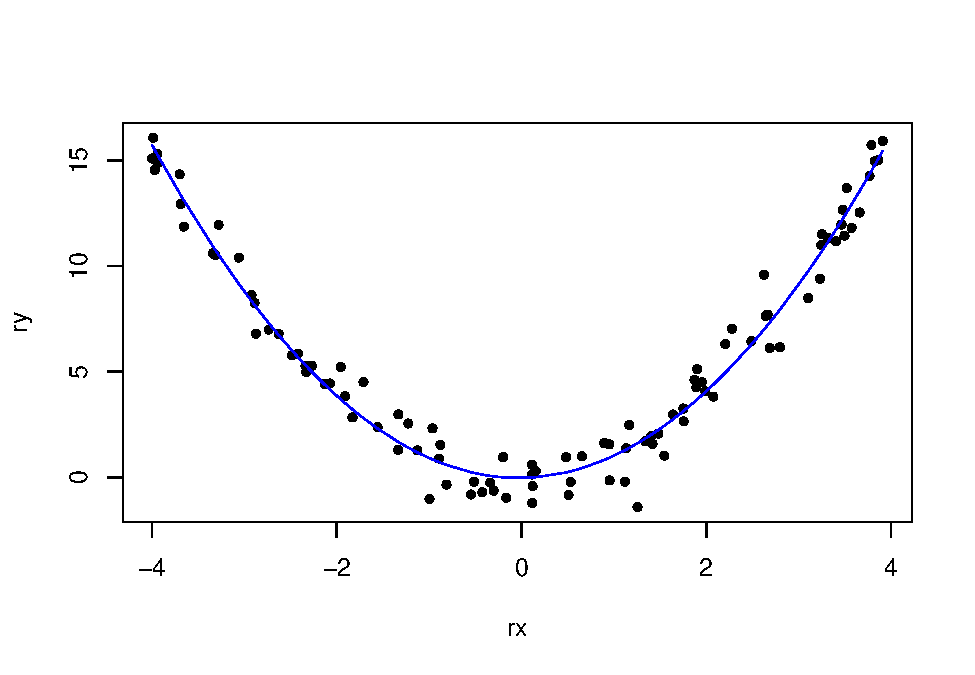
\includegraphics{_main_files/figure-latex/unnamed-chunk-24-1.pdf}

\begin{Shaded}
\begin{Highlighting}[]
\FunctionTok{set.seed}\NormalTok{(}\DecValTok{42}\NormalTok{)}
\NormalTok{rx }\OtherTok{\textless{}{-}} \FunctionTok{runif}\NormalTok{(}\DecValTok{1000}\NormalTok{,}\SpecialCharTok{{-}}\DecValTok{4}\NormalTok{,}\DecValTok{4}\NormalTok{)}
\NormalTok{rx }\OtherTok{\textless{}{-}} \FunctionTok{c}\NormalTok{(rx[rx }\SpecialCharTok{\textgreater{}=} \SpecialCharTok{{-}}\DecValTok{4} \SpecialCharTok{\&}\NormalTok{ rx }\SpecialCharTok{\textless{}} \SpecialCharTok{{-}}\DecValTok{3}\NormalTok{],rx[rx }\SpecialCharTok{\textgreater{}=} \SpecialCharTok{{-}}\DecValTok{3} \SpecialCharTok{\&}\NormalTok{ rx }\SpecialCharTok{\textless{}} \DecValTok{0}\NormalTok{],rx[rx}\SpecialCharTok{\textgreater{}=}\DecValTok{0} \SpecialCharTok{\&}\NormalTok{ rx }\SpecialCharTok{\textless{}} \DecValTok{2}\NormalTok{],rx[rx }\SpecialCharTok{\textgreater{}=} \DecValTok{2} \SpecialCharTok{\&}\NormalTok{ rx }\SpecialCharTok{\textless{}=} \DecValTok{4}\NormalTok{])}
\NormalTok{ry }\OtherTok{\textless{}{-}} \FunctionTok{c}\NormalTok{(}\DecValTok{3}\SpecialCharTok{*}\NormalTok{rx[rx}\SpecialCharTok{\textgreater{}=} \SpecialCharTok{{-}}\DecValTok{4} \SpecialCharTok{\&}\NormalTok{ rx}\SpecialCharTok{\textless{}} \SpecialCharTok{{-}}\DecValTok{3}\NormalTok{],}\SpecialCharTok{{-}}\DecValTok{4}\SpecialCharTok{*}\NormalTok{rx[rx}\SpecialCharTok{\textgreater{}=} \SpecialCharTok{{-}}\DecValTok{3} \SpecialCharTok{\&}\NormalTok{ rx}\SpecialCharTok{\textless{}} \DecValTok{0}\NormalTok{],}\FloatTok{0.2}\SpecialCharTok{*}\NormalTok{rx[rx }\SpecialCharTok{\textgreater{}=} \DecValTok{0} \SpecialCharTok{\&}\NormalTok{ rx}\SpecialCharTok{\textless{}}\DecValTok{2}\NormalTok{],}\DecValTok{6}\SpecialCharTok{*}\NormalTok{rx[rx}\SpecialCharTok{\textgreater{}=}\DecValTok{2} \SpecialCharTok{\&}\NormalTok{ rx}\SpecialCharTok{\textless{}=}\DecValTok{4}\NormalTok{])}
\NormalTok{ry }\OtherTok{\textless{}{-}}\NormalTok{ ry}\SpecialCharTok{+}\FunctionTok{rnorm}\NormalTok{(}\FunctionTok{length}\NormalTok{(ry),}\AttributeTok{sd=}\FloatTok{0.5}\NormalTok{)}
\FunctionTok{plot}\NormalTok{(rx,ry,}\AttributeTok{pch=}\DecValTok{20}\NormalTok{)}
\end{Highlighting}
\end{Shaded}

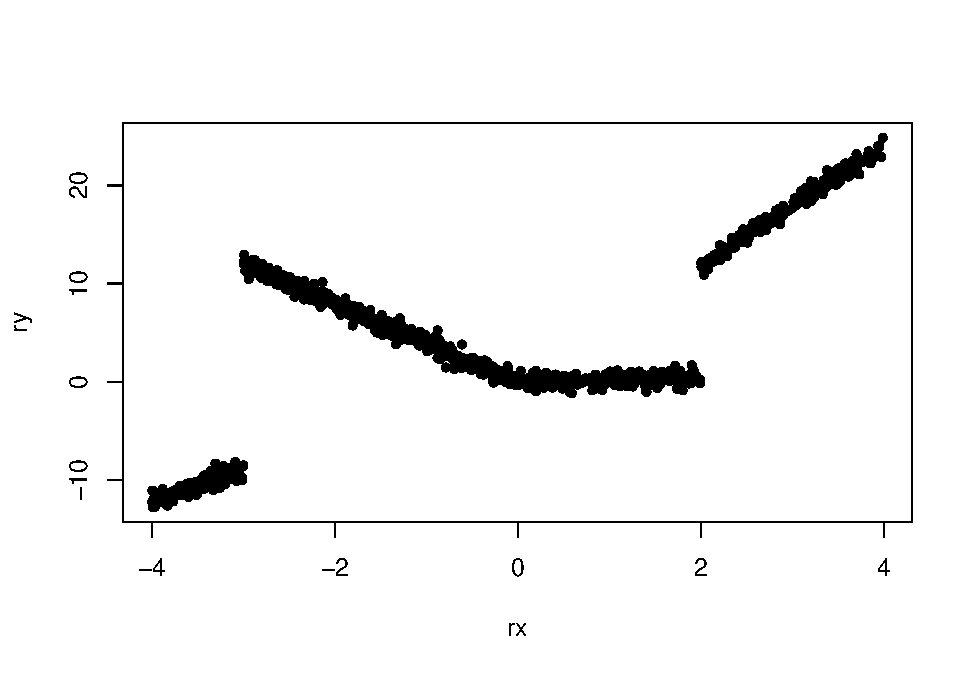
\includegraphics{_main_files/figure-latex/unnamed-chunk-25-1.pdf}

\begin{Shaded}
\begin{Highlighting}[]
\NormalTok{rr }\OtherTok{\textless{}{-}} \FunctionTok{lm}\NormalTok{(ry}\SpecialCharTok{\textasciitilde{}}\NormalTok{rx)}
\end{Highlighting}
\end{Shaded}

\begin{Shaded}
\begin{Highlighting}[]
\FunctionTok{library}\NormalTok{(splines)}
\NormalTok{a }\OtherTok{\textless{}{-}} \FunctionTok{lm}\NormalTok{(ry }\SpecialCharTok{\textasciitilde{}} \FunctionTok{ns}\NormalTok{(rx, }\AttributeTok{df =} \DecValTok{4}\NormalTok{))}
\FunctionTok{plot}\NormalTok{(rx,ry,}\AttributeTok{pch=}\DecValTok{20}\NormalTok{)}
\FunctionTok{points}\NormalTok{(rx[}\FunctionTok{order}\NormalTok{(rx)],}\FunctionTok{predict}\NormalTok{(a)[}\FunctionTok{order}\NormalTok{(rx)],}\AttributeTok{col=}\FunctionTok{rgb}\NormalTok{(}\DecValTok{0}\NormalTok{,}\DecValTok{0}\NormalTok{,}\DecValTok{1}\NormalTok{),}\AttributeTok{type=}\StringTok{"l"}\NormalTok{)}
\end{Highlighting}
\end{Shaded}

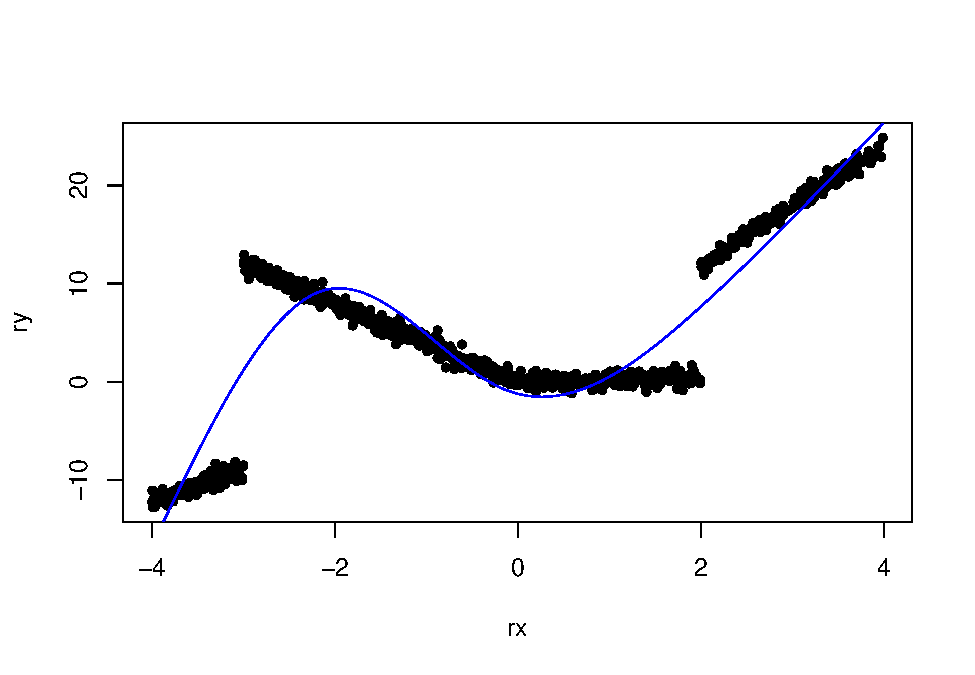
\includegraphics{_main_files/figure-latex/unnamed-chunk-26-1.pdf}

\hypertarget{covariances}{%
\section{Covariances}\label{covariances}}

Les covariances sont les carrées des écarts entre les valeurs prises par deux
variables aléatoires.

En fait ce sont les corrélations mais avec comme unités les unités naturelles
des deux variables et non des écart-types comme unités.

Cela peut être très utile quand on calcule des corrélations entre des grands
nombres et des petits nombre. Cela peut être difficile de \emph{lire} les covariances
donc on est amené à réduire les variables.

Par exemple :

Réduire les covariances équivaut à calculer la corrélation.

\hypertarget{tests}{%
\chapter{Tests}\label{tests}}

\hypertarget{convergence-vers-la-loi-normale}{%
\section{Convergence vers la loi normale}\label{convergence-vers-la-loi-normale}}

Si on tire des échantillons aléatoirement, alors la moyenne de ces échantillons
va converger vers une loi normale de moyenne \emph{m} et d'écat-type \emph{sigma}.

\href{https://datatrigger.shinyapps.io/CLT_Visualization/}{Central Limit Theorem}

\hypertarget{test-z}{%
\section{Test Z}\label{test-z}}

Le test Z est le calcul de la position de la loi normale par rapport à ces
quantiles.

On prend une variable que l'on centre/réduit si besoin. Alors si on moins de
\emph{xx} \% de chances que la moyenne se trouve entre les valeurs (positives et
négatives) des quantiles alors la différence entre la moyenne de la loi normale
réduite est différente de m, une valeur théorique fixée.

Schématiquement on utilise les quantiles de la loi normale. Si la moyenne se
distribue comme une loi normale alors, entre doit se trouver avec une confiance
de 95\% entre les deux quantiles qui \emph{englobe} 95\% des observations d'une loi
normale.

On a :

100 - 95 = 5\%

Comme on tient compte des observations à gauche et à droite
alors on a le quantile de 2,5\% à gauche et 97,5\% à droite.

\begin{Shaded}
\begin{Highlighting}[]
\NormalTok{y}\OtherTok{=}\FunctionTok{rnorm}\NormalTok{(}\DecValTok{1000000}\NormalTok{,}\DecValTok{0}\NormalTok{,}\DecValTok{1}\NormalTok{)}
\NormalTok{dd}\OtherTok{=}\FunctionTok{density}\NormalTok{(y)}
\FunctionTok{plot}\NormalTok{(dd,}\AttributeTok{main=}\StringTok{"Normale de moyenne 0"}\NormalTok{,}\AttributeTok{xlab=}\StringTok{"Valeurs de x"}\NormalTok{,}\AttributeTok{ylab=}\StringTok{"Densité"}\NormalTok{)}
\FunctionTok{abline}\NormalTok{(}\AttributeTok{v=}\DecValTok{0}\NormalTok{,}\AttributeTok{lty=}\DecValTok{3}\NormalTok{)}
\FunctionTok{abline}\NormalTok{(}\AttributeTok{v=}\DecValTok{0}\FloatTok{{-}1.96}\SpecialCharTok{*}\FunctionTok{sd}\NormalTok{(y),}\AttributeTok{lty=}\DecValTok{1}\NormalTok{,}\AttributeTok{col=}\FunctionTok{rgb}\NormalTok{(}\DecValTok{1}\NormalTok{,}\DecValTok{0}\NormalTok{,}\DecValTok{0}\NormalTok{,}\FloatTok{0.5}\NormalTok{))}
\FunctionTok{abline}\NormalTok{(}\AttributeTok{v=}\DecValTok{0}\FloatTok{+1.96}\SpecialCharTok{*}\FunctionTok{sd}\NormalTok{(y),}\AttributeTok{lty=}\DecValTok{1}\NormalTok{,}\AttributeTok{col=}\FunctionTok{rgb}\NormalTok{(}\DecValTok{1}\NormalTok{,}\DecValTok{0}\NormalTok{,}\DecValTok{0}\NormalTok{,}\FloatTok{0.5}\NormalTok{))}

\FunctionTok{polygon}\NormalTok{(}\FunctionTok{c}\NormalTok{(dd}\SpecialCharTok{$}\NormalTok{x[dd}\SpecialCharTok{$}\NormalTok{x}\SpecialCharTok{\textgreater{}{-}}\FloatTok{1.96} \SpecialCharTok{\&}\NormalTok{ dd}\SpecialCharTok{$}\NormalTok{x}\SpecialCharTok{\textless{}}\FloatTok{1.96}\NormalTok{],}\FunctionTok{rev}\NormalTok{(dd}\SpecialCharTok{$}\NormalTok{x[dd}\SpecialCharTok{$}\NormalTok{x}\SpecialCharTok{\textgreater{}} \SpecialCharTok{{-}}\FloatTok{1.96} \SpecialCharTok{\&}\NormalTok{ dd}\SpecialCharTok{$}\NormalTok{x}\SpecialCharTok{\textless{}}\FloatTok{1.96}\NormalTok{])),}\FunctionTok{c}\NormalTok{(}\FunctionTok{rep}\NormalTok{(}\DecValTok{0}\NormalTok{,}\FunctionTok{length}\NormalTok{(dd}\SpecialCharTok{$}\NormalTok{y))[dd}\SpecialCharTok{$}\NormalTok{x}\SpecialCharTok{\textgreater{}} \SpecialCharTok{{-}}\FloatTok{1.96} \SpecialCharTok{\&}\NormalTok{ dd}\SpecialCharTok{$}\NormalTok{x}\SpecialCharTok{\textless{}}\FloatTok{1.96}\NormalTok{],}\FunctionTok{rev}\NormalTok{(dd}\SpecialCharTok{$}\NormalTok{y[dd}\SpecialCharTok{$}\NormalTok{x}\SpecialCharTok{\textgreater{}} \SpecialCharTok{{-}}\FloatTok{1.96} \SpecialCharTok{\&}\NormalTok{ dd}\SpecialCharTok{$}\NormalTok{x}\SpecialCharTok{\textless{}}\FloatTok{1.96}\NormalTok{])),}\AttributeTok{col=}\FunctionTok{rgb}\NormalTok{(}\DecValTok{1}\NormalTok{,}\DecValTok{0}\NormalTok{,}\DecValTok{0}\NormalTok{,}\FloatTok{0.5}\NormalTok{))}
\end{Highlighting}
\end{Shaded}

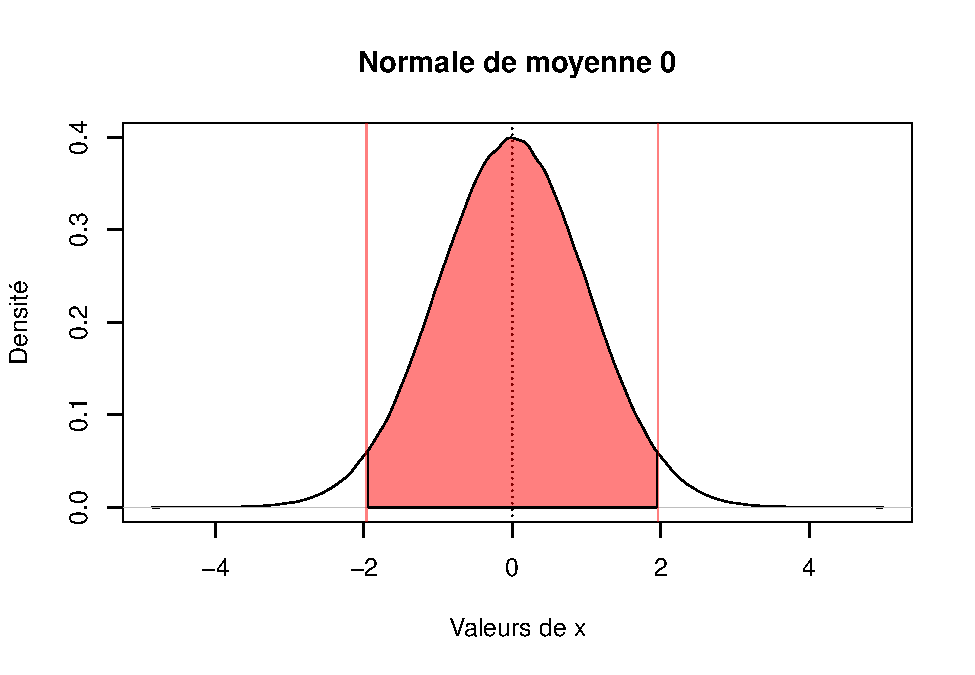
\includegraphics{_main_files/figure-latex/graphic1-1.pdf}

Le test est donc :

Si la distribution de la moyenne suit une loi normale centrée/réduite, sous
l'hypothèse nulle que \emph{m = m0} alors si \emph{m} est compris entre -1,96 et 1,96 alors
\emph{m} n'est pas différent de \emph{m0}.

Sinon \emph{m} est différent de \emph{m0} avec un seuil de 5\%.

\begin{Shaded}
\begin{Highlighting}[]
\FunctionTok{set.seed}\NormalTok{(}\DecValTok{42}\NormalTok{)}
\NormalTok{r0 }\OtherTok{\textless{}{-}} \FunctionTok{rnorm}\NormalTok{(}\DecValTok{100}\NormalTok{)}
\NormalTok{r1 }\OtherTok{\textless{}{-}} \FunctionTok{rnorm}\NormalTok{(}\DecValTok{100}\NormalTok{,}\AttributeTok{mean=}\FloatTok{0.25}\NormalTok{)}
\NormalTok{r3 }\OtherTok{\textless{}{-}} \FunctionTok{rnorm}\NormalTok{(}\DecValTok{100}\NormalTok{,}\AttributeTok{mean=}\FloatTok{0.5}\NormalTok{)}

\FunctionTok{plot}\NormalTok{(}\FunctionTok{density}\NormalTok{(r0),}\AttributeTok{xlim=}\FunctionTok{c}\NormalTok{(}\SpecialCharTok{{-}}\DecValTok{3}\NormalTok{,}\DecValTok{6}\NormalTok{),}\AttributeTok{ylim=}\FunctionTok{range}\NormalTok{(}\FunctionTok{c}\NormalTok{(}\FunctionTok{density}\NormalTok{(r0)}\SpecialCharTok{$}\NormalTok{y,}\FunctionTok{density}\NormalTok{(r1)}\SpecialCharTok{$}\NormalTok{y,}\FunctionTok{density}\NormalTok{(r3)}\SpecialCharTok{$}\NormalTok{y)))}
\FunctionTok{abline}\NormalTok{(}\AttributeTok{v=}\FunctionTok{mean}\NormalTok{(r0),}\AttributeTok{lty=}\DecValTok{2}\NormalTok{)}

\FunctionTok{points}\NormalTok{(}\FunctionTok{density}\NormalTok{(r1),}\AttributeTok{col=}\StringTok{"blue"}\NormalTok{,}\AttributeTok{type =} \StringTok{"l"}\NormalTok{)}
\FunctionTok{abline}\NormalTok{(}\AttributeTok{v=}\FunctionTok{mean}\NormalTok{(r1),}\AttributeTok{lty=}\DecValTok{2}\NormalTok{,}\AttributeTok{col=}\StringTok{"blue"}\NormalTok{)}

\FunctionTok{points}\NormalTok{(}\FunctionTok{density}\NormalTok{(r3),}\AttributeTok{col=}\StringTok{"green"}\NormalTok{,}\AttributeTok{type =} \StringTok{"l"}\NormalTok{)}
\FunctionTok{abline}\NormalTok{(}\AttributeTok{v=}\FunctionTok{mean}\NormalTok{(r3),}\AttributeTok{lty=}\DecValTok{2}\NormalTok{,}\AttributeTok{col=}\StringTok{"green"}\NormalTok{)}
\end{Highlighting}
\end{Shaded}

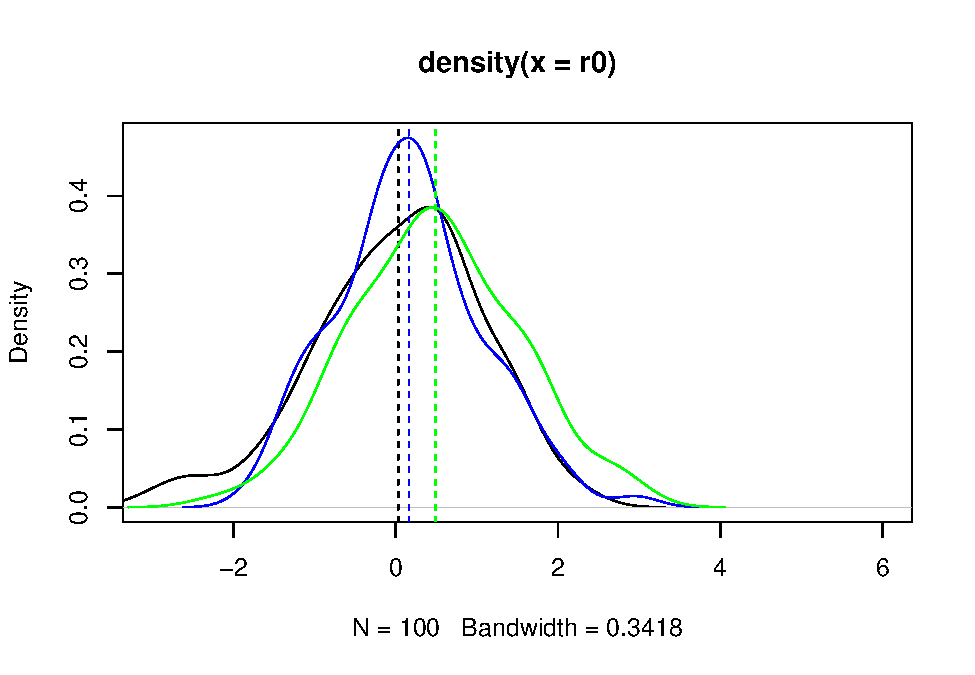
\includegraphics{_main_files/figure-latex/test_z1-1.pdf}

\begin{Shaded}
\begin{Highlighting}[]
\NormalTok{z }\OtherTok{\textless{}{-}} \FunctionTok{sqrt}\NormalTok{(}\FunctionTok{length}\NormalTok{(r1))}\SpecialCharTok{*}\NormalTok{(}\FunctionTok{mean}\NormalTok{(r1)}\SpecialCharTok{{-}}\DecValTok{0}\NormalTok{)}\SpecialCharTok{/}\FunctionTok{sd}\NormalTok{(r1)}
\NormalTok{z}
\end{Highlighting}
\end{Shaded}

\begin{verbatim}
## [1] 1.797402
\end{verbatim}

\begin{Shaded}
\begin{Highlighting}[]
\FunctionTok{abs}\NormalTok{(z) }\SpecialCharTok{\textgreater{}} \FloatTok{1.96}
\end{Highlighting}
\end{Shaded}

\begin{verbatim}
## [1] FALSE
\end{verbatim}

\begin{Shaded}
\begin{Highlighting}[]
\NormalTok{z }\OtherTok{\textless{}{-}} \FunctionTok{sqrt}\NormalTok{(}\FunctionTok{length}\NormalTok{(r3))}\SpecialCharTok{*}\NormalTok{(}\FunctionTok{mean}\NormalTok{(r3)}\SpecialCharTok{{-}}\DecValTok{0}\NormalTok{)}\SpecialCharTok{/}\FunctionTok{sd}\NormalTok{(r3)}
\NormalTok{z}
\end{Highlighting}
\end{Shaded}

\begin{verbatim}
## [1] 4.814414
\end{verbatim}

\begin{Shaded}
\begin{Highlighting}[]
\FunctionTok{abs}\NormalTok{(z) }\SpecialCharTok{\textgreater{}} \FloatTok{1.96}
\end{Highlighting}
\end{Shaded}

\begin{verbatim}
## [1] TRUE
\end{verbatim}

Question : que se passe-t-il si on fait un test seulement à droite ou seulement
à gauche ? C'est à dire si on s'intéresse non pas au cas où \emph{m} est autour de
\emph{m0} mais si m est plus grand que \emph{m0} ou plus petit que \emph{m0}.

\hypertarget{test-de-student}{%
\section{Test de Student}\label{test-de-student}}

Le test de Student est similaire au test Z, il est même identique dans certains
cas.

Les test de Student a deux fonctions :

\begin{itemize}
\item
  tester si une variable a une moyenne différente de m0.
\item
  test si les moyenne de deux variables sont différentes
\end{itemize}

On reconnait le premier cas qui est le test Z. D'ailleurs ont retrouve la même
valeur pour le test :

\begin{Shaded}
\begin{Highlighting}[]
\FunctionTok{t.test}\NormalTok{(r1)}
\end{Highlighting}
\end{Shaded}

\begin{verbatim}
## 
##  One Sample t-test
## 
## data:  r1
## t = 1.7974, df = 99, p-value = 0.07532
## alternative hypothesis: true mean is not equal to 0
## 95 percent confidence interval:
##  -0.01689135  0.34192394
## sample estimates:
## mean of x 
## 0.1625163
\end{verbatim}

Le test de Student est proche de l'ANOVA. En fait les résultats sont identiques
quand il y a l'argument \emph{var.equal=TRUE}.

Il signifie que les variances des variables sont identiques.

Un exemple du test de Student, n'est pas sur deux variable séparée mais entre
deux catégories d'individus qui forme chacun une population :

\begin{Shaded}
\begin{Highlighting}[]
\FunctionTok{t.test}\NormalTok{(}
\NormalTok{  iris}\SpecialCharTok{$}\NormalTok{Sepal.Length[iris}\SpecialCharTok{$}\NormalTok{Species}\SpecialCharTok{==}\StringTok{"setosa"}\NormalTok{],}
\NormalTok{  iris}\SpecialCharTok{$}\NormalTok{Sepal.Length[iris}\SpecialCharTok{$}\NormalTok{Species}\SpecialCharTok{==}\StringTok{"versicolor"}\NormalTok{],}
  \AttributeTok{var.equal =}\NormalTok{ T}
\NormalTok{)}
\end{Highlighting}
\end{Shaded}

\begin{verbatim}
## 
##  Two Sample t-test
## 
## data:  iris$Sepal.Length[iris$Species == "setosa"] and iris$Sepal.Length[iris$Species == "versicolor"]
## t = -10.521, df = 98, p-value < 2.2e-16
## alternative hypothesis: true difference in means is not equal to 0
## 95 percent confidence interval:
##  -1.1054165 -0.7545835
## sample estimates:
## mean of x mean of y 
##     5.006     5.936
\end{verbatim}

Le résultat est assez intuitif si on regarde le graphique des deux distributions :

\begin{Shaded}
\begin{Highlighting}[]
\FunctionTok{plot}\NormalTok{(}\FunctionTok{density}\NormalTok{(iris}\SpecialCharTok{$}\NormalTok{Sepal.Length[iris}\SpecialCharTok{$}\NormalTok{Species}\SpecialCharTok{==}\StringTok{"setosa"}\NormalTok{]),}\AttributeTok{type=}\StringTok{"l"}\NormalTok{,}\AttributeTok{main=}\StringTok{""}\NormalTok{,}
     \AttributeTok{xlab=}\StringTok{"Taille"}\NormalTok{,}\AttributeTok{ylab=}\StringTok{"Densité"}\NormalTok{)}
\FunctionTok{points}\NormalTok{(}\FunctionTok{density}\NormalTok{(iris}\SpecialCharTok{$}\NormalTok{Sepal.Length[iris}\SpecialCharTok{$}\NormalTok{Species}\SpecialCharTok{==}\StringTok{"versicolor"}\NormalTok{]),}\AttributeTok{type=}\StringTok{"l"}\NormalTok{,}\AttributeTok{col=}\StringTok{"blue"}\NormalTok{)}
\end{Highlighting}
\end{Shaded}

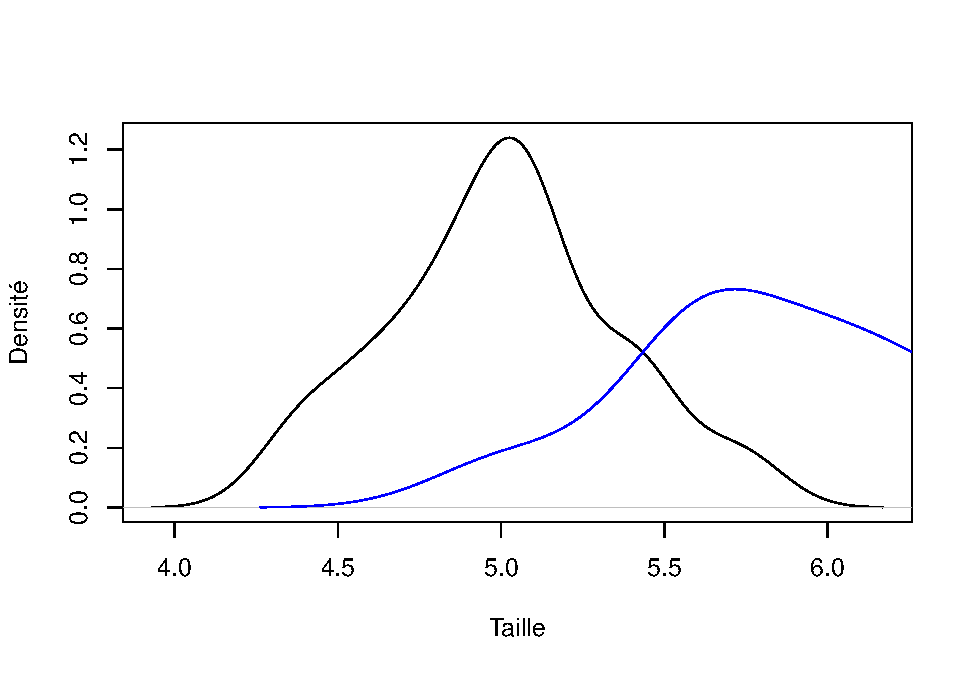
\includegraphics{_main_files/figure-latex/test_student1-1.pdf}

Pour résumer un test statistique est caractérisé :

\begin{itemize}
\item
  par des prérequis de travail (le plus souvent la normalité, égalité des
  variances, etc.).
\item
  des hypothèses pour le test qui définir les conclusions que l'on peut tirer du
  test. A votre niveau les hypothèses sont le plus souvent binaires.
  Oui/non : H0 contre H1.
\item
  le calcul de la valeur du test qui va être comparé aux ``tables'' de valeurs
\item
  le calcul des degrés de liberté
\item
  la conclusion du test : acceptation/rejet de H0 et idem pour H1.
\end{itemize}

Certaines statistiques dites ``bayésiennes'' fonctionnent différemment. Elles
touchent surtout la façon de définir et de calculer les tests.
La méthode décrite ici est appelé, à l'opposé de bayésiennes, la méthode
fréquentiste.

\hypertarget{erreur-de-type-i-et-ii}{%
\section{Erreur de Type I et II}\label{erreur-de-type-i-et-ii}}

L'erreur de type I est : une erreur de type I survient dans un test d'hypothèse
statistique lorsqu'une hypothèse nulle, qui est en réalité vraie, est rejetée
par erreur. Les erreurs de type I sont également connues sous le nom de ``faux
positifs'', elles représentent la détection d'un effet positif alors qu'il
n'existe aucun effet en réalité.

L'erreur de type II est : le risque de ne pas démontrer que deux groupes sont
différents alors qu'ils le sont dans la réalité.

La puissance est 1 - l'erreur de type II.

Par exemple, dans le cadre d'une étude randomisée en double aveugle pour le
développement d'un nouveau médicament, le risque de 2e espèce β peut être la
probabilité de conclure qu'un médicament n'est pas meilleur qu'un placebo alors
qu'il l'est. Dans ce cas, la puissance du test serait la probabilité de conclure
que le médicament est meilleur que le placébo, ce qui est vrai.

\hypertarget{tests-paramuxe9triques-et-non-paramuxe9triques}{%
\section{Tests ``paramétriques'' et non paramétriques}\label{tests-paramuxe9triques-et-non-paramuxe9triques}}

Dans le premier cas, tests paramétriques, ce sont les tests que l'on vient de
voir. Il repose sur des hypothèses de distribution : en l'occurence ici que
les données suivent une loi normale avec des paramètres : la moyenne et
l'écart-type. Le test ne ``fonctionne'' donc que dans le cas où ces trois
élements sont présents et corrects statistiquement.

Par exemple, si la distribution est très asymétrique, l'écart-type, la moyenne et
la loi normale ne sont pas au rendez-vous alors il faut se tourner vers d'autres
tests, en général des tests dits non-paramètriques.

Ces tests ne font pas d'hypothèse sur la distribution. Par exemple pour le test
de Student, l'équivalent est le test de Wilcoxon-Mann-Whitney.

Ce dernier pour illustrer le propos est basé sur les rangs des observations
plutôt que sur la valeur. Comme la médiane, cela rend le test plutôt robuste
à l'asymétrie et aux valeurs extrèmes.

L'inconvénient de ces tests est que pour un type I donné la puissance est plus
faible : on a des chances plus faibles de détecter un vrai positif qu'avec

\hypertarget{pruxe9cautions-uxe0-prendre-quand-on-travaille-avec-des-tests}{%
\section{Précautions à prendre quand on travaille avec des tests}\label{pruxe9cautions-uxe0-prendre-quand-on-travaille-avec-des-tests}}

\begin{itemize}
\item
  Ces préquis sont à \textbf{vérifier} avant de faire le test
\item
  Il faut comparer le nombre de degrés de liberté avec le nombre d'observations.
  En effet il y a des ``rules of thumb'' qui définissent le nombre de degrés de
  liberté en fonction du nombre d'observations. Par exemple pour les analyses
  structurales il faut de 20 à 40 observations minimums par degré de liberté.
\item
  Le choix est binaire. la p-value \textbf{ne donne pas de renseignements sur la
  ``force'' du test}.
\item
  Le choix de la valeur seuil de la \emph{p-value} doit être fait en amont et doit
  être contrôlé par des procédures statistiques si vous calculez de nombreux
  tests : cela s'appele correction de Bonferroni, Tukey, etc.
\end{itemize}

  \bibliography{book.bib,packages.bib}

\end{document}
